\section{2024年高考题}

\subsection{2024年全国甲卷（理）}\label{gk:2024年全国甲卷（理）}

\begin{description}
    \item[一、选择题] 本题共12小题，每小题5分，共60分．在每小题给出的四个选项中，只有一项是符合题目要求的．
    \begin{enumerate}[leftmargin=5pt]
        \item 若 $z=5+\i$，则 $\i(\bar{z}+z)=$
       
        {\centering\begin{tabular*}{\linewidth}{@{}@{\extracolsep{\fill}}llll@{}}
          \(\text{A. }10\i\)  & \(\text{B. }2\i\)  & \(\text{C. }10\)  & \(\text{D. }2\)
        \end{tabular*}\par}

        \item 已知集合 $A=\{1,2,3,4,5,9\}$，$B=\{x\mid\sqrt{x}\in A\}$，则 $\complement_A(A\cap B)=$
       
        {\centering\begin{tabular*}{\linewidth}{@{}@{\extracolsep{\fill}}llll@{}}
          \(\text{A. }\{1,4,9\}\)  & \(\text{B. }\{3,4,9\}\)  & \(\text{C. }\{1,2,3\}\)  & \(\text{D. }\{2,3,5\}\)
        \end{tabular*}\par}

        \item 若 $x,y$ 满足约束条件 $\begin{cases}4x-3y-3\geqslant0,\\x-2y-2\leqslant0,\\2x+6y-9\leqslant0,\end{cases}$ 则 $z=x-5y$ 的最小值为
        
        {\centering\begin{tabular*}{\linewidth}{@{}@{\extracolsep{\fill}}llll@{}}
          \(\text{A. }\dfrac{1}{2}\)  & \(\text{B. }0\)  & \(\text{C. }-\dfrac{5}{2}\)  & \(\text{D. }-\dfrac{7}{2}\)
        \end{tabular*}\par}

        \item 记 $S_n$ 为等差数列 $\{a_n\}$ 的前 $n$ 项和．已知 $S_5=S_{10}$，$a_5=1$，则 $a_1=$
       
        {\centering\begin{tabular*}{\linewidth}{@{}@{\extracolsep{\fill}}llll@{}}
          \(\text{A. }\dfrac{7}{2}\)  & \(\text{B. }\dfrac{7}{3}\)  & \(\text{C. }-\dfrac{1}{3}\)  & \(\text{D. }-\dfrac{7}{11}\)
        \end{tabular*}\par}

        \item 已知双曲线的两个焦点分别为 $(0,4)$，$(0,-4)$，点 $(-6,4)$ 在该双曲线上，则该双曲线的离心率为
       
        {\centering\begin{tabular*}{\linewidth}{@{}@{\extracolsep{\fill}}llll@{}}
          \(\text{A. }4\)  & \(\text{B. }3\)  & \(\text{C. }2\)  & \(\text{D. }\sqrt{2}\)
        \end{tabular*}\par}

        \item 设函数 $f(x)=\dfrac{\mathrm{e}^x+2\sin x}{1+x^2}$，则曲线 $y=f(x)$ 在点 $(0,1)$ 处的切线与两坐标轴所围成的三角形的面积为
       
        {\centering\begin{tabular*}{\linewidth}{@{}@{\extracolsep{\fill}}llll@{}}
          \(\text{A. }\dfrac{1}{6}\)  & \(\text{B. }\dfrac{1}{3}\)  & \(\text{C. }\dfrac{1}{2}\)  & \(\text{D. }\dfrac{2}{3}\)
        \end{tabular*}\par}

        \item 函数 $y=-x^2+(\mathrm{e}^x-\mathrm{e}^{-x})\sin x$ 在区间 $[-2.8,2.8]$ 的图象大致为
        
        {\centering
            \begin{tabular*}{\linewidth}{@{}@{\extracolsep{\fill}}cccc@{}}
            \(\text{A. }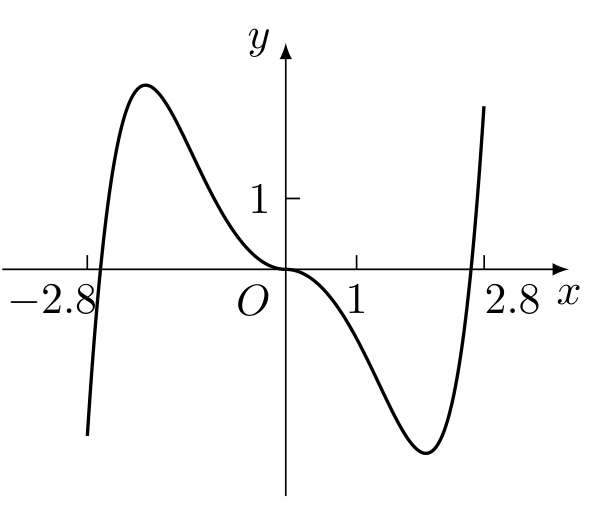
\includegraphics[width=0.15\paperwidth]{GaoKao/images/2024/national_paper_a_science/q7_optA.png}\)  &  \(\text{B. }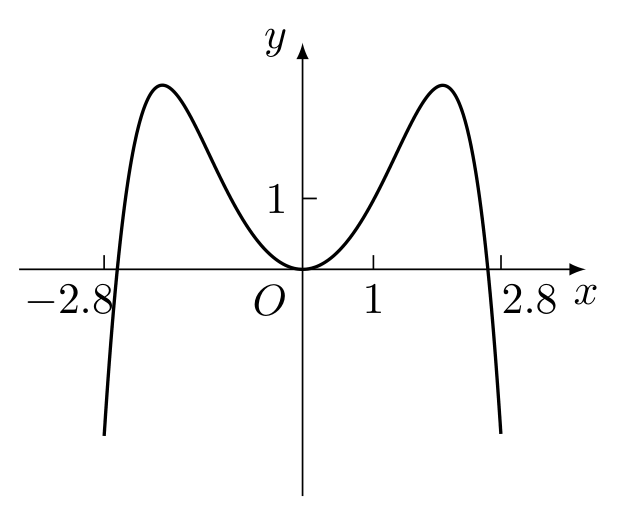
\includegraphics[width=0.15\paperwidth]{GaoKao/images/2024/national_paper_a_science/q7_optB.png}\)  &  \(\text{C. }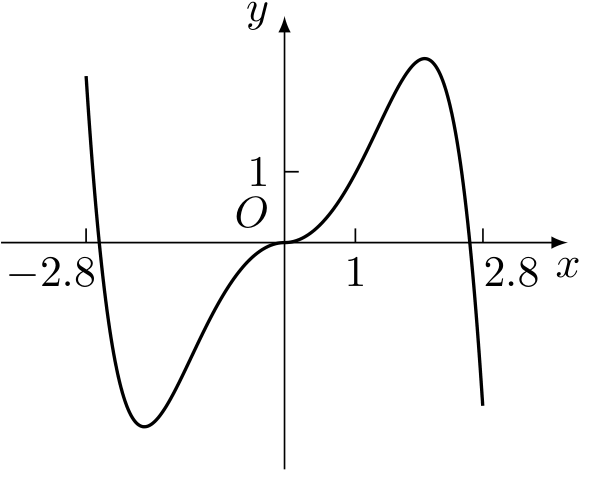
\includegraphics[width=0.15\paperwidth]{GaoKao/images/2024/national_paper_a_science/q7_optC.png}\)  &  \(\text{D. }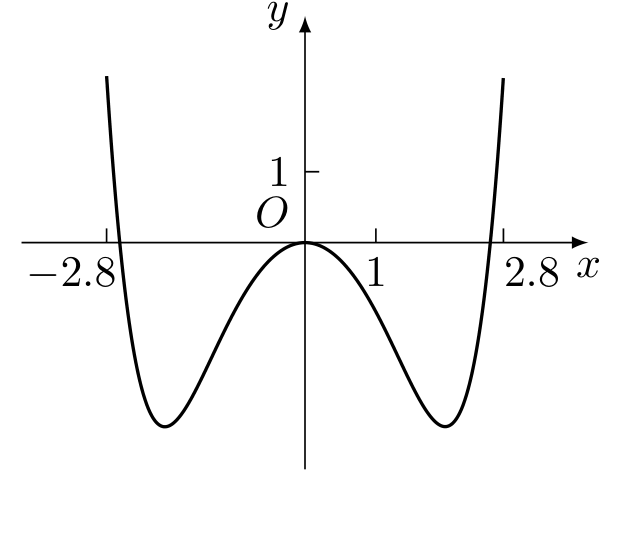
\includegraphics[width=0.15\paperwidth]{GaoKao/images/2024/national_paper_a_science/q7_optD.png}\)
        \end{tabular*}
        \par}

        \item 已知 $\dfrac{\cos\alpha}{\cos\alpha-\sin\alpha}=\sqrt{3}$，则 $\tan\bigl(\alpha+\dfrac{\pi}{4}\bigr)=$
       
        {\centering\begin{tabular*}{\linewidth}{@{}@{\extracolsep{\fill}}llll@{}}
          \(\text{A. }2\sqrt{3}+1\)  & \(\text{B. }2\sqrt{3}-1\)  & \(\text{C. }\dfrac{\sqrt{3}}{2}\)  & \(\text{D. }1-\sqrt{3}\)
        \end{tabular*}\par}

        \item 设向量 $\bm a=(x+1,x)$，$\bm b=(x,2)$，则
        
        {\centering\begin{tabular*}{\linewidth}{@{}@{\extracolsep{\fill}}llll@{}}
          \(\text{A. }x=-3\) 是 $\bm a\perp\bm b$ 的必要条件 \\
          \(\text{B. }x=1+\sqrt{3}$ 是 $\bm a\parallel\bm b$ 的必要条件 \\
          \(\text{C. }x=0$ 是 $\bm a\perp\bm b$ 的充分条件 \\
          \(\text{D. }x=-1+\sqrt{3}$ 是 $\bm a\parallel\bm b$ 的充分条件
        \end{tabular*}\par}

        \item 设 $\alpha,\beta$ 为两个平面，$m,n$ 为两条直线，且 $\alpha\cap\beta=m$．下述四个命题：
        
        \ding{172}若 $m\parallel n$，则 $n\parallel\alpha$ 或 $n\parallel\beta$；
        
        \ding{173}若 $m\perp n$，则 $n\perp\alpha$ 或 $n\perp\beta$；
        
        \ding{174}若 $n\parallel\alpha$ 且 $n\parallel\beta$，则 $m\parallel n$；
        
        \ding{175}若 $n$ 与 $\alpha,\beta$ 所成的角相等，则 $m\perp n$．
        
        其中所有真命题的编号是
       
        {\centering\begin{tabular*}{\linewidth}{@{}@{\extracolsep{\fill}}llll@{}}
          \(\text{A. }\)\ding{172}\ding{174}  & \(\text{B. }\)\ding{173}\ding{175}  & \(\text{C. }\)\ding{172}\ding{173}\ding{174}  & \(\text{D. }\)\ding{172}\ding{174}\ding{175}
        \end{tabular*}\par}

        \item 记 $\triangle ABC$ 的内角 $A,B,C$ 的对边分别为 $a,b,c$，已知 $B=60^\circ$，$b^2=\dfrac{9}{4}ac$，则 $\sin A+\sin C=$
       
        {\centering\begin{tabular*}{\linewidth}{@{}@{\extracolsep{\fill}}llll@{}}
          \(\text{A. }\dfrac{3}{2}\)  & \(\text{B. }\sqrt{2}\)  & \(\text{C. }\dfrac{\sqrt{7}}{2}\)  & \(\text{D. }\dfrac{\sqrt{3}}{2}\)
        \end{tabular*}\par}

        \item 已知 $b$ 是 $a,c$ 的等差中项，直线 $ax+by+c=0$ 与圆 $x^2+y^2+4y-1=0$ 交于 $A,B$ 两点，则 $|AB|$ 的最小值为
       
        {\centering\begin{tabular*}{\linewidth}{@{}@{\extracolsep{\fill}}llll@{}}
          \(\text{A. }1\)  & \(\text{B. }2\)  & \(\text{C. }4\)  & \(\text{D. }2\sqrt{5}\)
        \end{tabular*}\par}
    \end{enumerate}
\end{description}

\begin{description}
    \item[二、填空题] 本题共4小题，每小题5分，共20分．
    \begin{enumerate}[leftmargin=5pt]
      \addtocounter{enumi}{+12}
        \item $\bigl(\dfrac{1}{3}+x\bigr)^{10}$ 的展开式中，各项系数中的最大值为 \rule[-0.3ex]{3em}{0.4pt}．
        \item 已知圆台甲、乙的上底面半径均为 $r_1$，下底面半径均为 $r_2$，圆台甲、乙的母线长分别为 $2(r_2-r_1)$，$3(r_2-r_1)$，则圆台甲与乙的体积之比为 \rule[-0.3ex]{3em}{0.4pt}．
        \item 已知 $a>1$ 且 $\dfrac{1}{\log_8 a}-\dfrac{1}{\log_a 4}=-\dfrac{5}{2}$，则 $a=$ \rule[-0.3ex]{3em}{0.4pt}．
        \item 有6个相同的球，分别标有数字1，2，3，4，5，6，从中无放回地随机取3次，每次取1个球．设 $m$ 为前两次取出的球上数字的平均值，$n$ 为取出的三个球上数字的平均值，则 $m$ 与 $n$ 之差的绝对值不大于 $\dfrac{1}{2}$ 的概率为 \rule[-0.3ex]{3em}{0.4pt}．
    \end{enumerate}
\end{description}

\begin{description}
    \item[三、解答题] 本题共7小题，共70分．解答应写出文字说明、证明过程或演算步骤．第17\textasciitilde21题为必考题，第22、23题为选考题．
    \begin{enumerate}[leftmargin=5pt]
      \addtocounter{enumi}{+16}
        \item （12分）

        某工厂进行生产线智能化升级改造．升级改造后，从该工厂甲、乙两个车间的产品中随机抽取150件进行检验，数据如下：

        {\centering\begin{tabular}{c|c|c|c|c}
        \hline
        & 优级品 & 合格品 & 不合格品 & 总计 \\
        \hline
        甲车间 & 26 & 24 & 0 & 50 \\
        \hline
        乙车间 & 70 & 28 & 2 & 100 \\
        \hline
        总计 & 96 & 52 & 2 & 150 \\
        \hline
        \end{tabular}\par}

        \begin{enumerate}[label=(\arabic*)]
            \item 填写如下列联表，能否有 $95\%$ 的把握认为甲、乙两车间产品的优级品率存在差异？能否有 $99\%$ 的把握认为甲、乙两车间产品的优级品率存在差异？

            {\centering\begin{tabular}{c|c|c}
            \hline
            & 优级品 & 非优级品 \\
            \hline
            甲车间 & & \\
            \hline
            乙车间 & & \\
            \hline
            \end{tabular}\par}

            附：$K^2=\dfrac{n(ad-bc)^2}{(a+b)(c+d)(a+c)(b+d)}$，
            {\begin{tabular}{c|ccc}
            \hline
            $P(K^2\geqslant k)$ & 0.050 & 0.010 & 0.001 \\
            \hline
            $k$ & 3.841 & 6.635 & 10.828 \\
            \hline
            \end{tabular}\par}

            \item 已知升级改造前该工厂产品的优级品率 $p=0.5$．设 $\bar{p}$ 为升级改造后抽取的 $n$ 件产品的优级品率，如果 $\bar{p}>p+1.65\sqrt{\frac{p(1-p)}{n}}$，则认为该工厂产品的优级品率提高了．根据抽取的150件产品的数据，能否认为生产线智能化升级改造后，该工厂产品的优级品率提高了？$(\sqrt{150}\approx12.247)$
        \end{enumerate}

        \item （12分）

        记 $S_n$ 为数列 $\{a_n\}$ 的前 $n$ 项和，已知 $4S_n=3a_n+4$．

        \begin{enumerate}[label=(\arabic*)]
            \item 求 $\{a_n\}$ 的通项公式；
            \item 设 $b_n=(-1)^{n-1}na_n$，求数列 $\{b_n\}$ 的前 $n$ 项和 $T_n$．
        \end{enumerate}

        \item （12分）

        如图，在以 $A,B,C,D,E,F$ 为顶点的五面体中，四边形 $ABCD$ 与四边形 $ADEF$ 均为等腰梯形，$EF\parallel AD$，$BC\parallel AD$，$AD=4$，$AB=BC=EF=2$，$ED=\sqrt{10}$，$FB=2\sqrt{3}$，$M$ 为 $AD$ 的中点．

        {\centering
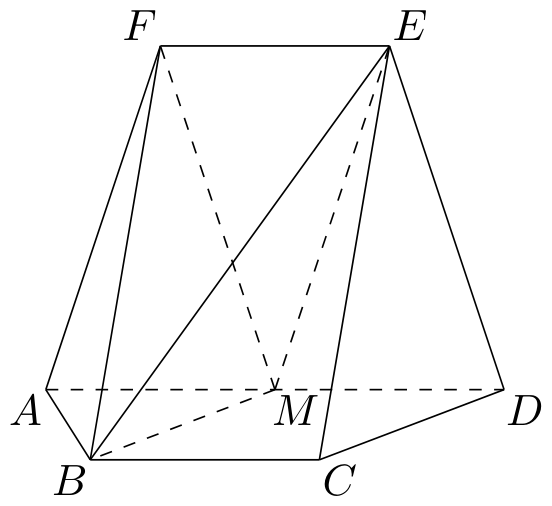
\includegraphics[width=6.9cm]{GaoKao/images/2024/national_paper_a_science/q19_fig1.png}
\par}

        \begin{enumerate}[label=(\arabic*)]
            \item 证明：$BM\parallel$ 平面 $CDE$；
            \item 求二面角 $F$-$BM$-$E$ 的正弦值．
        \end{enumerate}

        \item （12分）

        设椭圆 $C:\dfrac{x^2}{a^2}+\dfrac{y^2}{b^2}=1\,(a>b>0)$ 的右焦点为 $F$，点 $M\bigl(1,\frac{3}{2}\bigr)$ 在 $C$ 上，且 $MF\perp x$ 轴．

        \begin{enumerate}[label=(\arabic*)]
            \item 求 $C$ 的方程；
            \item 过点 $P(4,0)$ 的直线交 $C$ 于 $A,B$ 两点，$N$ 为线段 $FP$ 的中点，直线 $NB$ 交直线 $MF$ 于点 $Q$，证明：$AQ\perp y$ 轴．
        \end{enumerate}

        \item （12分）

        已知函数 $f(x)=(1-ax)\ln(1+x)-x$．

        \begin{enumerate}[label=(\arabic*)]
            \item 若 $a=-2$，求 $f(x)$ 的极值；
            \item 当 $x\geqslant0$ 时，$f(x)\geqslant0$，求 $a$ 的取值范围．
        \end{enumerate}

        \item （10分）[选修4-4：坐标系与参数方程]

        在直角坐标系 $xOy$ 中，以坐标原点为极点，$x$ 轴正半轴为极轴建立极坐标系，曲线 $C$ 的极坐标方程为 $\rho=\rho\cos\theta+1$．

        \begin{enumerate}[label=(\arabic*)]
            \item 写出 $C$ 的直角坐标方程；
            \item 设直线 $l:\begin{cases}x=t,\\y=t+a\end{cases}$（$t$ 为参数），若 $C$ 与 $l$ 相交于 $A,B$ 两点，且 $|AB|=2$，求 $a$．
        \end{enumerate}

        \item （10分）[选修4-5：不等式选讲]

        已知实数 $a,b$ 满足 $a+b\geqslant3$．

        \begin{enumerate}[label=(\arabic*)]
            \item 证明：$2a^2+2b^2>a+b$；
            \item 证明：$|a-2b^2|+|b-2a^2|\geqslant6$．
        \end{enumerate}
    \end{enumerate}
\end{description}
\clearpage


\subsection{2024年全国甲卷（文）}\label{gk:2024年全国甲卷（文）}

\begin{description}
    \item[一、选择题] 本题共12小题，每小题5分，共60分．在每小题给出的四个选项中，只有一项是符合题目要求的．
    \begin{enumerate}[leftmargin=5pt]
        \item 若 $z=\sqrt{2}\i$，则 $z\bar{z}=$
       
        {\centering\begin{tabular*}{\linewidth}{@{}@{\extracolsep{\fill}}llll@{}}
          \(\text{A. }-2\)  & \(\text{B. }-\sqrt{2}\)  & \(\text{C. }\sqrt{2}\)  & \(\text{D. }2\)
        \end{tabular*}\par}

        \item 已知集合 $A=\{1,2,3,4,5,9\}$，$B=\{x\mid x+1\in A\}$，则 $A\cap B=$
       
        {\centering\begin{tabular*}{\linewidth}{@{}@{\extracolsep{\fill}}llll@{}}
          \(\text{A. }\{1,2,3\}\)  & \(\text{B. }\{3,4,9\}\)  & \(\text{C. }\{1,2,3,4\}\)  & \(\text{D. }\{2,3,4,5\}\)
        \end{tabular*}\par}

        \item 设向量 $\bm a=(x+1,x)$，$\bm b=(x,2)$，$\bm c=(1,1)$，若 $\bm a-2\bm b$ 与 $\bm c$ 共线，则 $x=$
       
        {\centering\begin{tabular*}{\linewidth}{@{}@{\extracolsep{\fill}}llll@{}}
          \(\text{A. }\dfrac{5}{2}\)  & \(\text{B. }\dfrac{1}{2}\)  & \(\text{C. }-\dfrac{1}{2}\)  & \(\text{D. }-\dfrac{5}{2}\)
        \end{tabular*}\par}

        \item 某独唱比赛的决赛阶段共有甲、乙、丙、丁四人参加，每人出场一次，出场次序由随机抽签确定．则丙不是第一个出场，且甲或乙最后出场的概率是
       
        {\centering\begin{tabular*}{\linewidth}{@{}@{\extracolsep{\fill}}llll@{}}
          \(\text{A. }\dfrac{1}{6}\)  & \(\text{B. }\dfrac{1}{4}\)  & \(\text{C. }\dfrac{1}{3}\)  & \(\text{D. }\dfrac{1}{2}\)
        \end{tabular*}\par}

        \item 记 $S_n$ 为等差数列 $\{a_n\}$ 的前 $n$ 项和．已知 $S_9=1$，则 $a_3+a_7=$
       
        {\centering\begin{tabular*}{\linewidth}{@{}@{\extracolsep{\fill}}llll@{}}
          \(\text{A. }\dfrac{1}{9}\)  & \(\text{B. }\dfrac{2}{9}\)  & \(\text{C. }\dfrac{1}{3}\)  & \(\text{D. }\dfrac{2}{3}\)
        \end{tabular*}\par}

        \item 已知双曲线的两个焦点分别为 $(0,4)$，$(0,-4)$，点 $(-6,4)$ 在该双曲线上，则该双曲线的离心率为
       
        {\centering\begin{tabular*}{\linewidth}{@{}@{\extracolsep{\fill}}llll@{}}
          \(\text{A. }4\)  & \(\text{B. }3\)  & \(\text{C. }2\)  & \(\text{D. }\sqrt{2}\)
        \end{tabular*}\par}

        \item 设函数 $f(x)=\dfrac{\mathrm{e}^x+2\sin x}{1+x^2}$，则曲线 $y=f(x)$ 在点 $(0,1)$ 处的切线与两坐标轴所围成的三角形的面积为
       
        {\centering\begin{tabular*}{\linewidth}{@{}@{\extracolsep{\fill}}llll@{}}
          \(\text{A. }\dfrac{1}{6}\)  & \(\text{B. }\dfrac{1}{3}\)  & \(\text{C. }\dfrac{1}{2}\)  & \(\text{D. }\dfrac{2}{3}\)
        \end{tabular*}\par}

        \item 函数 $y=-x^2+(\mathrm{e}^x-\mathrm{e}^{-x})\sin x$ 在区间 $[-2.8,2.8]$ 的图象大致为
        
        {\centering
            \begin{tabular*}{\linewidth}{@{}@{\extracolsep{\fill}}cccc@{}}
            \(\text{A. }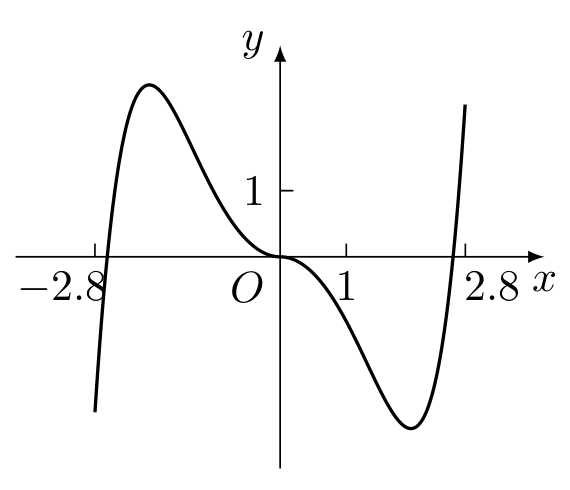
\includegraphics[width=0.15\paperwidth]{GaoKao/images/2024/national_paper_a_liberal/q8_optA.png}\)  &  \(\text{B. }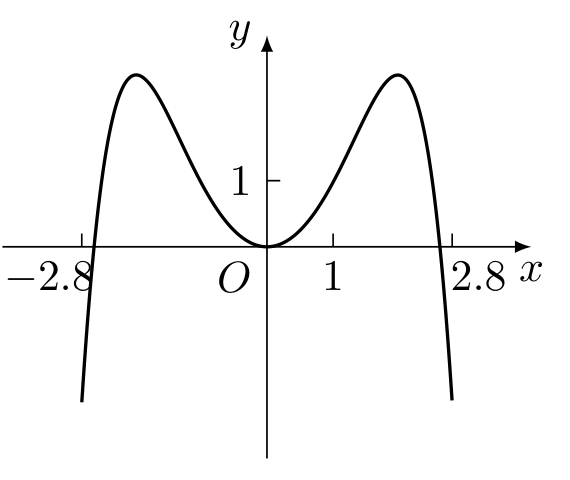
\includegraphics[width=0.15\paperwidth]{GaoKao/images/2024/national_paper_a_liberal/q8_optB.png}\)  &  \(\text{C. }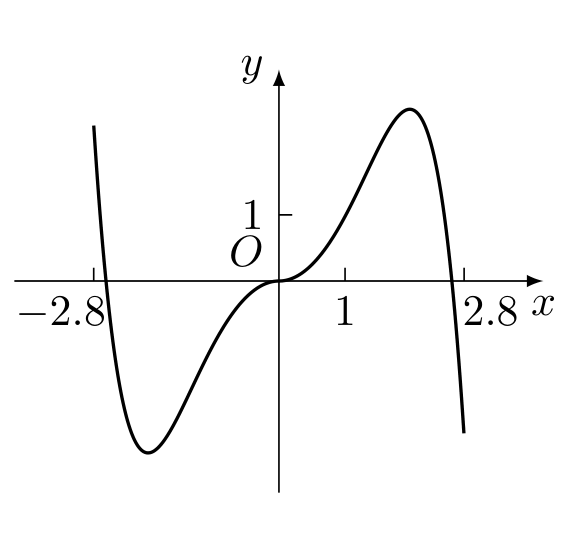
\includegraphics[width=0.15\paperwidth]{GaoKao/images/2024/national_paper_a_liberal/q8_optC.png}\)  &  \(\text{D. }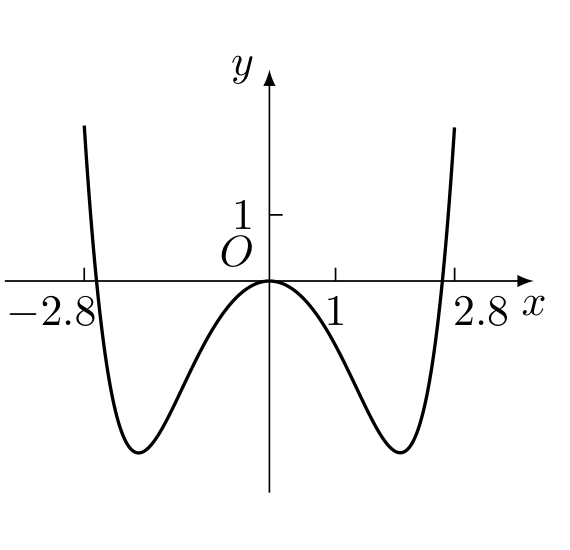
\includegraphics[width=0.15\paperwidth]{GaoKao/images/2024/national_paper_a_liberal/q8_optD.png}\)
        \end{tabular*}
        \par}

        \item 直线 $2x-y-2=0$ 与圆 $x^2+y^2-6x-8y=0$ 交于 $A,B$ 两点，则 $|AB|=$
       
        {\centering\begin{tabular*}{\linewidth}{@{}@{\extracolsep{\fill}}llll@{}}
          \(\text{A. }4\)  & \(\text{B. }5\)  & \(\text{C. }8\)  & \(\text{D. }10\)
        \end{tabular*}\par}

        \item 已知 $\dfrac{\cos\alpha}{\cos\alpha-\sin\alpha}=\sqrt{3}$，则 $\tan\bigl(\alpha+\dfrac{\pi}{4}\bigr)=$
       
        {\centering\begin{tabular*}{\linewidth}{@{}@{\extracolsep{\fill}}llll@{}}
          \(\text{A. }2\sqrt{3}+1\)  & \(\text{B. }2\sqrt{3}-1\)  & \(\text{C. }\dfrac{\sqrt{3}}{2}\)  & \(\text{D. }1-\sqrt{3}\)
        \end{tabular*}\par}

        \item 设 $\alpha,\beta$ 为两个平面，$m,n$ 为两条直线，且 $\alpha\cap\beta=m$．下述四个命题：
        
        \ding{172}若 $m\parallel n$，则 $n\parallel\alpha$ 或 $n\parallel\beta$；
        
        \ding{173}若 $m\perp n$，则 $n\perp\alpha$ 或 $n\perp\beta$；
        
        \ding{174}若 $n\parallel\alpha$ 且 $n\parallel\beta$，则 $m\parallel n$；
        
        \ding{175}若 $n$ 与 $\alpha,\beta$ 所成的角相等，则 $m\perp n$．
        
        其中所有真命题的编号是
       
        {\centering\begin{tabular*}{\linewidth}{@{}@{\extracolsep{\fill}}llll@{}}
          \(\text{A. }\)\ding{172}\ding{174}  & \(\text{B. }\)\ding{173}\ding{175}  & \(\text{C. }\)\ding{172}\ding{173}\ding{174}  & \(\text{D. }\)\ding{172}\ding{174}\ding{175}
        \end{tabular*}\par}

        \item 记 $\triangle ABC$ 的内角 $A,B,C$ 的对边分别为 $a,b,c$，已知 $B=60^\circ$，$b^2=\dfrac{9}{4}ac$，则 $\sin A+\sin C=$
       
        {\centering\begin{tabular*}{\linewidth}{@{}@{\extracolsep{\fill}}llll@{}}
          \(\text{A. }\dfrac{3}{2}\)  & \(\text{B. }\sqrt{2}\)  & \(\text{C. }\dfrac{\sqrt{7}}{2}\)  & \(\text{D. }\dfrac{\sqrt{3}}{2}\)
        \end{tabular*}\par}
    \end{enumerate}
\end{description}

\begin{description}
    \item[二、填空题] 本题共4小题，每小题5分，共20分．
    \begin{enumerate}[leftmargin=5pt]
      \addtocounter{enumi}{+12}
        \item 函数 $f(x)=\sin x-\sqrt{3}\cos x$ 在区间 $[0,\pi]$ 的最大值为 \rule[-0.3ex]{3em}{0.4pt}．
        \item 已知圆台甲、乙的上底面半径均为 $r_1$，下底面半径均为 $r_2$，圆台甲、乙的母线长分别为 $2(r_2-r_1)$，$3(r_2-r_1)$，则圆台甲与乙的体积之比为 \rule[-0.3ex]{3em}{0.4pt}．
        \item 已知 $a>1$ 且 $\dfrac{1}{\log_8 a}-\dfrac{1}{\log_a 4}=-\dfrac{5}{2}$，则 $a=$ \rule[-0.3ex]{3em}{0.4pt}．
        \item 当 $x>0$ 时，曲线 $y=x^3-3x$ 与曲线 $y=-(x-1)^2+a$ 有两个交点，则 $a$ 的取值范围是 \rule[-0.3ex]{3em}{0.4pt}．
    \end{enumerate}
\end{description}

\begin{description}
    \item[三、解答题] 本题共7小题，共70分．解答应写出文字说明、证明过程或演算步骤．第17\textasciitilde21题为必考题，第22、23题为选考题．
    \begin{enumerate}[leftmargin=5pt]
      \addtocounter{enumi}{+16}
        \item （12分）

        记 $S_n$ 为等比数列 $\{a_n\}$ 的前 $n$ 项和，已知 $2S_n=3a_{n+1}-3$．

        \begin{enumerate}[label=(\arabic*)]
            \item 求 $\{a_n\}$ 的通项公式；
            \item 求数列 $\{S_n\}$ 的前 $n$ 项和．
        \end{enumerate}

        \item （12分）

        某工厂进行生产线智能化升级改造．升级改造后，从该工厂甲、乙两个车间的产品中随机抽取150件进行检验，数据如下：

        {\centering\begin{tabular}{c|c|c|c|c}
        \hline
        & 优级品 & 合格品 & 不合格品 & 总计 \\
        \hline
        甲车间 & 26 & 24 & 0 & 50 \\
        \hline
        乙车间 & 70 & 28 & 2 & 100 \\
        \hline
        总计 & 96 & 52 & 2 & 150 \\
        \hline
        \end{tabular}\par}

        \begin{enumerate}[label=(\arabic*)]
            \item 填写如下列联表，能否有 $95\%$ 的把握认为甲、乙两车间产品的优级品率存在差异？能否有 $99\%$ 的把握认为甲、乙两车间产品的优级品率存在差异？

            附：$K^2=\dfrac{n(ad-bc)^2}{(a+b)(c+d)(a+c)(b+d)}$，
            $P(K^2\geqslant k)$：0.050--3.841，0.010--6.635，0.001--10.828．

            \item 已知升级改造前该工厂产品的优级品率 $p=0.5$．设 $\bar{p}$ 为升级改造后抽取的 $n$ 件产品的优级品率，如果 $\bar{p}>p+1.65\sqrt{\frac{p(1-p)}{n}}$，则认为该工厂产品的优级品率提高了．根据抽取的150件产品的数据，能否认为生产线智能化升级改造后，该工厂产品的优级品率提高了？$(\sqrt{150}\approx12.247)$
        \end{enumerate}

        \item （12分）

        如图，在以 $A,B,C,D,E,F$ 为顶点的五面体中，四边形 $ABCD$ 与四边形 $ADEF$ 均为等腰梯形，$EF\parallel AD$，$BC\parallel AD$，$AD=4$，$AB=BC=EF=2$，$ED=\sqrt{10}$，$FB=2\sqrt{3}$，$M$ 为 $AD$ 的中点．

        {\centering
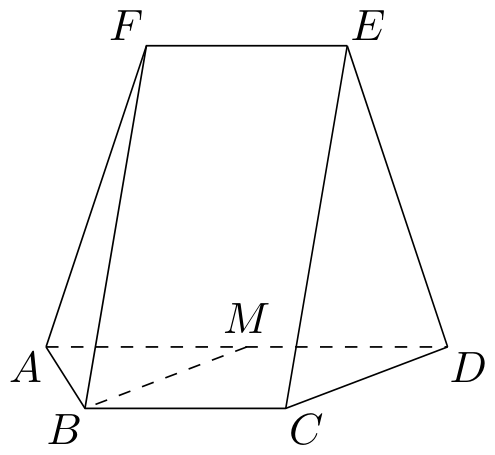
\includegraphics[width=6.1cm]{GaoKao/images/2024/national_paper_a_liberal/q19_fig1.png}
\par}

        \begin{enumerate}[label=(\arabic*)]
            \item 证明：$BM\parallel$ 平面 $CDE$；
            \item 求 $M$ 到平面 $FAB$ 的距离．
        \end{enumerate}

        \item （12分）

        已知函数 $f(x)=a(x-1)-\ln x+1$．

        \begin{enumerate}[label=(\arabic*)]
            \item 讨论 $f(x)$ 的单调性；
            \item 设 $a\leqslant2$，证明：当 $x>1$ 时，$f(x)<\mathrm{e}^{x-1}$．
        \end{enumerate}

        \item （12分）

        设椭圆 $C:\dfrac{x^2}{a^2}+\dfrac{y^2}{b^2}=1\,(a>b>0)$ 的右焦点为 $F$，点 $M\bigl(1,\frac{3}{2}\bigr)$ 在 $C$ 上，且 $MF\perp x$ 轴．

        \begin{enumerate}[label=(\arabic*)]
            \item 求 $C$ 的方程；
            \item 过点 $P(4,0)$ 的直线交 $C$ 于 $A,B$ 两点，$N$ 为线段 $FP$ 的中点，直线 $NB$ 交直线 $MF$ 于点 $Q$，证明：$AQ\perp y$ 轴．
        \end{enumerate}

        \item （10分）[选修4-4：坐标系与参数方程]

        在直角坐标系 $xOy$ 中，以坐标原点为极点，$x$ 轴正半轴为极轴建立极坐标系，曲线 $C$ 的极坐标方程为 $\rho=\rho\cos\theta+1$．

        \begin{enumerate}[label=(\arabic*)]
            \item 写出 $C$ 的直角坐标方程；
            \item 设直线 $l:\begin{cases}x=t,\\y=t+a\end{cases}$（$t$ 为参数），若 $C$ 与 $l$ 相交于 $A,B$ 两点，且 $|AB|=2$，求 $a$．
        \end{enumerate}

        \item （10分）[选修4-5：不等式选讲]

        已知实数 $a,b$ 满足 $a+b\geqslant3$．

        \begin{enumerate}[label=(\arabic*)]
            \item 证明：$2a^2+2b^2>a+b$；
            \item 证明：$|a-2b^2|+|b-2a^2|\geqslant6$．
        \end{enumerate}
    \end{enumerate}
\end{description}
\clearpage


\subsection{2024年新高考I卷}\label{gk:2024年新高考I卷}

\begin{description}
    \item[一、选择题] 本题共8小题，每小题5分，共40分．在每小题给出的四个选项中，只有一项是符合题目要求的．
    \begin{enumerate}[leftmargin=5pt]
        \item 已知集合 $A=\{x\mid -5<x^3<5\}$，$B=\{-3,-1,0,2,3\}$，则 $A\cap B=$
       
        {\centering\begin{tabular*}{\linewidth}{@{}@{\extracolsep{\fill}}llll@{}}
          \(\text{A. }\{-1,0\}\)  & \(\text{B. }\{2,3\}\)  & \(\text{C. }\{-3,-1,0\}\)  & \(\text{D. }\{-1,0,2\}\)
        \end{tabular*}\par}

        \item 若 $\dfrac{z}{z-1}=1+\i$，则 $z=$
       
        {\centering\begin{tabular*}{\linewidth}{@{}@{\extracolsep{\fill}}llll@{}}
          \(\text{A. }-1-\i\)  & \(\text{B. }-1+\i\)  & \(\text{C. }1-\i\)  & \(\text{D. }1+\i\)
        \end{tabular*}\par}

        \item 已知向量 $\bm a=(0,1)$，$\bm b=(2,x)$，若 $\bm b\perp(\bm b-4\bm a)$，则 $x=$
       
        {\centering\begin{tabular*}{\linewidth}{@{}@{\extracolsep{\fill}}llll@{}}
          \(\text{A. }-2\)  & \(\text{B. }-1\)  & \(\text{C. }1\)  & \(\text{D. }2\)
        \end{tabular*}\par}

        \item 已知 $\cos(\alpha+\beta)=m$，$\tan\alpha\tan\beta=2$，则 $\cos(\alpha-\beta)=$
       
        {\centering\begin{tabular*}{\linewidth}{@{}@{\extracolsep{\fill}}llll@{}}
          \(\text{A. }-3m\)  & \(\text{B. }-\dfrac{m}{3}\)  & \(\text{C. }\dfrac{m}{3}\)  & \(\text{D. }3m\)
        \end{tabular*}\par}

        \item 已知圆柱和圆锥的底面半径相等，侧面积相等，且它们的高均为 $\sqrt{3}$，则圆锥的体积为
       
        {\centering\begin{tabular*}{\linewidth}{@{}@{\extracolsep{\fill}}llll@{}}
          \(\text{A. }2\sqrt{3}\pi\)  & \(\text{B. }3\sqrt{3}\pi\)  & \(\text{C. }6\sqrt{3}\pi\)  & \(\text{D. }9\sqrt{3}\pi\)
        \end{tabular*}\par}

        \item 已知函数 $f(x)=\begin{cases}-x^2-2ax-a,&x<0,\\\mathrm{e}^x+\ln(x+1),&x\geqslant0,\end{cases}$ 在 $\mathbb{R}$ 上单调递增，则 $a$ 的取值范围是
       
        {\centering\begin{tabular*}{\linewidth}{@{}@{\extracolsep{\fill}}llll@{}}
          \(\text{A. }(-\infty,0]\)  & \(\text{B. }[-1,0]\)  & \(\text{C. }[-1,1]\)  & \(\text{D. }[0,+\infty)\)
        \end{tabular*}\par}

        \item 当 $x\in[0,2\pi]$ 时，曲线 $y=\sin x$ 与 $y=2\sin\bigl(3x-\frac{\pi}{6}\bigr)$ 的交点个数为
       
        {\centering\begin{tabular*}{\linewidth}{@{}@{\extracolsep{\fill}}llll@{}}
          \(\text{A. }3\)  & \(\text{B. }4\)  & \(\text{C. }6\)  & \(\text{D. }8\)
        \end{tabular*}\par}

        \item 已知函数 $f(x)$ 的定义域为 $\mathbb{R}$，$f(x)>f(x-1)+f(x-2)$，且当 $x<3$ 时 $f(x)=x$，则下列结论中一定正确的是
       
        {\centering\begin{tabular*}{\linewidth}{@{}@{\extracolsep{\fill}}llll@{}}
          \(\text{A. }f(10)>100\)  & \(\text{B. }f(20)>1000\)  & \(\text{C. }f(10)<1000\)  & \(\text{D. }f(20)<10000\)
        \end{tabular*}\par}
    \end{enumerate}
\end{description}

\begin{description}
    \item[二、选择题] 本题共3小题，每小题6分，共18分．在每小题给出的选项中，有多项符合题目要求．全部选对的得6分，部分选对的得部分分，有选错的得0分．
    \begin{enumerate}[leftmargin=5pt]
      \addtocounter{enumi}{+8}
        \item 随着"一带一路"国际合作的深入，某茶叶种植区多措并举推动茶叶出口．为了解推动出口后的亩收入（单位：万元）情况，从该种植区抽取样本，得到推动出口后亩收入的样本均值 $\bar{x}=2.1$，样本方差 $s^2=0.01$．已知该种植区以往的亩收入 $X$ 服从正态分布 $N(1.8,0.1^2)$，假设推动出口后的亩收入 $Y$ 服从正态分布 $N(\bar{x},s^2)$，则（若随机变量 $Z$ 服从正态分布 $N(\mu,\sigma^2)$，则 $P(Z<\mu+\sigma)\approx0.8413$）
        \begin{enumerate}[label=\Alph*.]
            \item $P(X>2)>0.2$
            \item $P(X>2)<0.5$
            \item $P(Y>2)>0.5$
            \item $P(Y>2)<0.8$
        \end{enumerate}

        \item 设函数 $f(x)=(x-1)^2(x-4)$，则
        \begin{enumerate}[label=\Alph*.]
            \item $x=3$ 是 $f(x)$ 的极小值点
            \item 当 $0<x<1$ 时，$f(x)<f(x^2)$
            \item 当 $1<x<2$ 时，$-4<f(2x-1)<0$
            \item 当 $-1<x<0$ 时，$f(2-x)>f(x)$
        \end{enumerate}

        \item 设计一条美丽的丝带，其造型可以看作图中曲线 $C$ 的一部分．已知 $C$ 过坐标原点 $O$，且 $C$ 上的点满足：横坐标大于 $-2$；到点 $F(2,0)$ 的距离与到定直线 $x=a\,(a<0)$ 的距离之积为 $4$．则
        \begin{enumerate}[label=\Alph*.]
            \item $a=-2$
            \item 点 $(2\sqrt{2},0)$ 在 $C$ 上
            \item $C$ 在第一象限的点的纵坐标的最大值为 $1$
            \item 当点 $(x_0,y_0)$ 在 $C$ 上时，$y_0\leqslant\dfrac{4}{x_0+2}$
        \end{enumerate}
    \end{enumerate}
\end{description}

\begin{description}
    \item[三、填空题] 本题共3小题，每小题5分，共15分．
    \begin{enumerate}[leftmargin=5pt]
      \addtocounter{enumi}{+11}
        \item 设双曲线 $C:\dfrac{x^2}{a^2}-\dfrac{y^2}{b^2}=1\,(a>0,b>0)$ 的左、右焦点分别为 $F_1,F_2$，过 $F_2$ 作平行于 $y$ 轴的直线交 $C$ 于 $A,B$ 两点．若 $|F_1A|=13$，$|AB|=10$，则 $C$ 的离心率为 \rule[-0.3ex]{3em}{0.4pt}．
        \item 若曲线 $y=\mathrm{e}^x+x$ 在点 $(0,1)$ 处的切线也是曲线 $y=\ln(x+1)+a$ 的切线，则 $a=$ \rule[-0.3ex]{3em}{0.4pt}．
        \item 甲、乙两人各有四张卡片，每张卡片上标有一个数字，甲的卡片上分别标有数字1，3，5，7，乙的卡片上分别标有数字2，4，6，8，两人进行四轮比赛．在每轮比赛中，两人各自从自己持有的卡片中随机选一张，并比较所选卡片上数字的大小，数字大的人得1分，数字小的人得0分，然后各自弃置此轮所选的卡片（弃置的卡片在此后的轮次中不能使用）．则四轮比赛后，甲的总得分不小于2的概率为 \rule[-0.3ex]{3em}{0.4pt}．
    \end{enumerate}
\end{description}

\begin{description}
    \item[四、解答题] 本题共5小题，共77分．解答应写出文字说明、证明过程或演算步骤．
    \begin{enumerate}[leftmargin=5pt]
      \addtocounter{enumi}{+14}
        \item （13分）

        记 $\triangle ABC$ 的内角 $A,B,C$ 的对边分别为 $a,b,c$．已知 $\sin C=\sqrt{2}\cos B$，$a^2+b^2-c^2=\sqrt{2}ab$．

        \begin{enumerate}[label=(\arabic*)]
            \item 求 $B$；
            \item 若 $\triangle ABC$ 的面积为 $3+\sqrt{3}$，求 $c$．
        \end{enumerate}

        \item （15分）

        已知 $A(0,3)$ 和 $P\bigl(3,\frac{3}{2}\bigr)$ 为椭圆 $C:\dfrac{x^2}{a^2}+\dfrac{y^2}{b^2}=1\,(a>b>0)$ 上两点．

        \begin{enumerate}[label=(\arabic*)]
            \item 求 $C$ 的离心率；
            \item 若过 $P$ 的直线 $l$ 交 $C$ 于另一点 $B$，且 $\triangle ABP$ 的面积为 $9$，求 $l$ 的方程．
        \end{enumerate}

        \item （15分）

        如图，四棱锥 $P$-$ABCD$ 中，$PA\perp$ 底面 $ABCD$，$PA=AC=2$，$BC=1$，$AB=\sqrt{3}$．

        {\centering
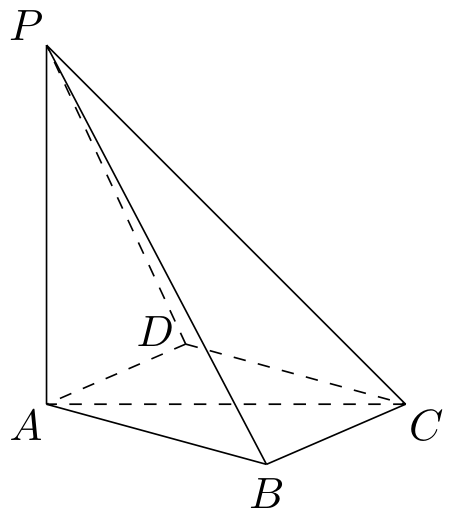
\includegraphics[width=5.3cm]{GaoKao/images/2024/new_gaokao_paper_1/q17_fig1.png}
\par}

        \begin{enumerate}[label=(\arabic*)]
            \item 若 $AD\perp PB$，证明：$AD\parallel$ 平面 $PBC$；
            \item 若 $AD\perp DC$，且二面角 $A$-$CP$-$D$ 的正弦值为 $\dfrac{\sqrt{42}}{7}$，求 $AD$．
        \end{enumerate}

        \item （17分）

        已知函数 $f(x)=\ln\dfrac{x}{2-x}+ax+b(x-1)^3$．

        \begin{enumerate}[label=(\arabic*)]
            \item 若 $b=0$，且 $f'(x)\geqslant0$，求 $a$ 的最小值；
            \item 证明：曲线 $y=f(x)$ 是中心对称图形；
            \item 若 $f(x)>-2$ 当且仅当 $1<x<2$，求 $b$ 的取值范围．
        \end{enumerate}

        \item （17分）

        设 $m$ 为正整数，数列 $a_1,a_2,\cdots,a_{4m+2}$ 是公差不为 $0$ 的等差数列，若从中删去两项 $a_i$ 和 $a_j\,(i<j)$ 后剩余的 $4m$ 项可被平均分为 $m$ 组，且每组的 $4$ 个数都能构成等差数列，则称数列 $a_1,a_2,\cdots,a_{4m+2}$ 是 $(i,j)$-可分数列．

        \begin{enumerate}[label=(\arabic*)]
            \item 写出所有的 $(i,j),1\leqslant i<j\leqslant6$，使得数列 $a_1,a_2,\cdots,a_6$ 是 $(i,j)$-可分数列；
            \item 当 $m\geqslant3$ 时，证明：数列 $a_1,a_2,\cdots,a_{4m+2}$ 是 $(2,13)$-可分数列；
            \item 从 $1,2,\cdots,4m+2$ 中一次任取两个数 $i$ 和 $j\,(i<j)$，记数列 $a_1,a_2,\cdots,a_{4m+2}$ 是 $(i,j)$-可分数列的概率为 $P_m$，证明：$P_m>\dfrac{1}{8}$．
        \end{enumerate}
    \end{enumerate}
\end{description}
\clearpage


\subsection{2024年新高考II卷}\label{gk:2024年新高考II卷}

\begin{description}
    \item[一、选择题] 本题共8小题，每小题5分，共40分．在每小题给出的四个选项中，只有一项是符合题目要求的．
    \begin{enumerate}[leftmargin=5pt]
        \item 已知 $z=-1-\i$，则 $|z|=$
       
        {\centering\begin{tabular*}{\linewidth}{@{}@{\extracolsep{\fill}}llll@{}}
          \(\text{A. }0\)  & \(\text{B. }1\)  & \(\text{C. }\sqrt{2}\)  & \(\text{D. }2\)
        \end{tabular*}\par}

        \item 已知命题 $p:\forall x\in\mathbb{R},|x+1|>1$；命题 $q:\exists x>0,x^3=x$．则
        
        {\centering\begin{tabular*}{\linewidth}{@{}@{\extracolsep{\fill}}llll@{}}
          \(\text{A. }p\) 和 $q$ 都是真命题  & \(\text{B. }\neg p\) 和 $q$ 都是真命题 \\
          \(\text{C. }p\) 和 $\neg q$ 都是真命题  & \(\text{D. }\neg p\) 和 $\neg q$ 都是真命题
        \end{tabular*}\par}

        \item 已知向量 $\bm a,\bm b$ 满足 $|\bm a|=1$，$|\bm a+2\bm b|=2$，且 $(\bm b-2\bm a)\perp\bm b$，则 $|\bm b|=$
       
        {\centering\begin{tabular*}{\linewidth}{@{}@{\extracolsep{\fill}}llll@{}}
          \(\text{A. }\dfrac{1}{2}\)  & \(\text{B. }\dfrac{\sqrt{2}}{2}\)  & \(\text{C. }\dfrac{\sqrt{3}}{2}\)  & \(\text{D. }1\)
        \end{tabular*}\par}

        \item 某农业研究部门在面积相等的100块稻田上种植一种新型水稻，得到各块稻田的亩产量（单位：kg）并整理得下表：

        {\centering\begin{tabular}{c|c|c|c|c|c|c}
        \hline
        亩产量 & $[900,950)$ & $[950,1000)$ & $[1000,1050)$ & $[1050,1100)$ & $[1100,1150)$ & $[1150,1200)$ \\
        \hline
        频数 & 6 & 12 & 18 & 30 & 24 & 10 \\
        \hline
        \end{tabular}\par}

        根据表中数据，下列结论中正确的是
        
        {\centering\begin{tabular*}{\linewidth}{@{}@{\extracolsep{\fill}}llll@{}}
          \(\text{A. }\)100块稻田亩产量的中位数小于1050\,kg \\
          \(\text{B. }\)100块稻田中亩产量低于1100\,kg的稻田所占比例超过$80\%$ \\
          \(\text{C. }\)100块稻田亩产量的极差介于200\,kg至300\,kg之间 \\
          \(\text{D. }\)100块稻田亩产量的平均值介于900\,kg至1000\,kg之间
        \end{tabular*}\par}

        \item 已知曲线 $C:x^2+y^2=16\,(y>0)$，从 $C$ 上任意一点 $P$ 向 $x$ 轴作垂线段 $PP'$，$P'$ 为垂足，则线段 $PP'$ 的中点 $M$ 的轨迹方程为
        
        {\centering\begin{tabular*}{\linewidth}{@{}@{\extracolsep{\fill}}llll@{}}
          \(\text{A. }\dfrac{x^2}{16}+\dfrac{y^2}{4}=1\,(y>0)\)  & \(\text{B. }\dfrac{x^2}{16}+\dfrac{y^2}{8}=1\,(y>0)\) \\
          \(\text{C. }\dfrac{y^2}{16}+\dfrac{x^2}{4}=1\,(y>0)\)  & \(\text{D. }\dfrac{y^2}{16}+\dfrac{x^2}{8}=1\,(y>0)\)
        \end{tabular*}\par}

        \item 设函数 $f(x)=a(x+1)^2-1$，$g(x)=\cos x+2ax$．当 $x\in(-1,1)$ 时，曲线 $y=f(x)$ 与 $y=g(x)$ 恰有一个交点，则 $a=$
       
        {\centering\begin{tabular*}{\linewidth}{@{}@{\extracolsep{\fill}}llll@{}}
          \(\text{A. }-1\)  & \(\text{B. }\dfrac{1}{2}\)  & \(\text{C. }1\)  & \(\text{D. }2\)
        \end{tabular*}\par}

        \item 已知正三棱台 $ABC$-$A_1B_1C_1$ 的体积为 $\dfrac{52}{3}$，$AB=6$，$A_1B_1=2$，则 $A_1A$ 与平面 $ABC$ 所成角的正切值为
       
        {\centering\begin{tabular*}{\linewidth}{@{}@{\extracolsep{\fill}}llll@{}}
          \(\text{A. }\dfrac{1}{2}\)  & \(\text{B. }1\)  & \(\text{C. }2\)  & \(\text{D. }3\)
        \end{tabular*}\par}

        \item 设函数 $f(x)=(x+a)\ln(x+b)$．若 $f(x)\geqslant0$，则 $a^2+b^2$ 的最小值为
       
        {\centering\begin{tabular*}{\linewidth}{@{}@{\extracolsep{\fill}}llll@{}}
          \(\text{A. }\dfrac{1}{8}\)  & \(\text{B. }\dfrac{1}{4}\)  & \(\text{C. }\dfrac{1}{2}\)  & \(\text{D. }1\)
        \end{tabular*}\par}
    \end{enumerate}
\end{description}

\begin{description}
    \item[二、选择题] 本题共3小题，每小题6分，共18分．在每小题给出的选项中，有多项符合题目要求．全部选对的得6分，部分选对的得部分分，有选错的得0分．
    \begin{enumerate}[leftmargin=5pt]
      \addtocounter{enumi}{+8}
        \item 对于函数 $f(x)=\sin2x$ 和 $g(x)=\sin\bigl(2x-\frac{\pi}{4}\bigr)$，下列说法中正确的有
        \begin{enumerate}[label=\Alph*.]
            \item $f(x)$ 与 $g(x)$ 有相同的零点
            \item $f(x)$ 与 $g(x)$ 有相同的最大值
            \item $f(x)$ 与 $g(x)$ 有相同的最小正周期
            \item $f(x)$ 与 $g(x)$ 的图象有相同的对称轴
        \end{enumerate}

        \item 抛物线 $C:y^2=4x$ 的准线为 $l$，$P$ 为 $C$ 上动点．过 $P$ 作 $\odot A:x^2+(y-4)^2=1$ 的一条切线，$Q$ 为切点．过 $P$ 作 $l$ 的垂线，垂足为 $B$．则
        \begin{enumerate}[label=\Alph*.]
            \item $l$ 与 $\odot A$ 相切
            \item 当 $P,A,B$ 三点共线时，$|PQ|=\sqrt{15}$
            \item 当 $|PB|=2$ 时，$PA\perp AB$
            \item 满足 $|PA|=|PB|$ 的点 $P$ 有且仅有 $2$ 个
        \end{enumerate}

        \item 设函数 $f(x)=2x^3-3ax^2+1$，则
        \begin{enumerate}[label=\Alph*.]
            \item 当 $a>1$ 时，$f(x)$ 有三个零点
            \item 当 $a<0$ 时，$x=0$ 是 $f(x)$ 的极大值点
            \item 存在 $a,b$，使得 $x=b$ 为曲线 $y=f(x)$ 的对称轴
            \item 存在 $a$，使得点 $(1,f(1))$ 为曲线 $y=f(x)$ 的对称中心
        \end{enumerate}
    \end{enumerate}
\end{description}

\begin{description}
    \item[三、填空题] 本题共3小题，每小题5分，共15分．
    \begin{enumerate}[leftmargin=5pt]
      \addtocounter{enumi}{+11}
        \item 记 $S_n$ 为等差数列 $\{a_n\}$ 的前 $n$ 项和．若 $a_3+a_4=7$，$3a_2+a_5=5$，则 $S_{10}=$ \rule[-0.3ex]{3em}{0.4pt}．
        \item 已知 $\alpha$ 为第一象限角，$\beta$ 为第三象限角，$\tan\alpha+\tan\beta=4$，$\tan\alpha\tan\beta=\sqrt{2}+1$，则 $\sin(\alpha+\beta)=$ \rule[-0.3ex]{3em}{0.4pt}．
        \item 在如图的 $4\times4$ 的方格表中选 $4$ 个方格，要求每行和每列均恰有一个方格被选中，则共有 \rule[-0.3ex]{3em}{0.4pt} 种选法．在所有符合上述要求的选法中，选中方格中的 $4$ 个数之和的最大值是 \rule[-0.3ex]{3em}{0.4pt}．

        {\centering\begin{tabular}{c|c|c|c}
        \hline
        11 & 21 & 31 & 40 \\
        \hline
        12 & 22 & 33 & 42 \\
        \hline
        13 & 22 & 33 & 43 \\
        \hline
        15 & 24 & 34 & 44 \\
        \hline
        \end{tabular}\par}
    \end{enumerate}
\end{description}

\begin{description}
    \item[四、解答题] 本题共5小题，共77分．解答应写出文字说明、证明过程或演算步骤．
    \begin{enumerate}[leftmargin=5pt]
      \addtocounter{enumi}{+14}
        \item （13分）

        记 $\triangle ABC$ 的内角 $A,B,C$ 的对边分别为 $a,b,c$，已知 $\sin A+\sqrt{3}\cos A=2$．

        \begin{enumerate}[label=(\arabic*)]
            \item 求 $A$；
            \item 若 $a=2$，$\sqrt{2}b\sin C=c\sin2B$，求 $\triangle ABC$ 的周长．
        \end{enumerate}

        \item （15分）

        已知函数 $f(x)=\mathrm{e}^x-ax-a^3$．

        \begin{enumerate}[label=(\arabic*)]
            \item 当 $a=1$ 时，求曲线 $y=f(x)$ 在点 $(1,f(1))$ 处的切线方程；
            \item 若 $f(x)$ 有极小值，且极小值小于 $0$，求 $a$ 的取值范围．
        \end{enumerate}

        \item （15分）

        如图，平面四边形 $ABCD$ 中，$AB=8$，$CD=3$，$AD=5\sqrt{3}$，$\angle ADC=90^\circ$，$\angle BAD=30^\circ$，点 $E,F$ 满足 $\overrightarrow{AE}=\frac{2}{5}\overrightarrow{AD}$，$\overrightarrow{AF}=\frac{1}{2}\overrightarrow{AB}$，将 $\triangle AEF$ 沿 $EF$ 翻折至 $\triangle PEF$，使得 $PC=4\sqrt{3}$．

        {\centering
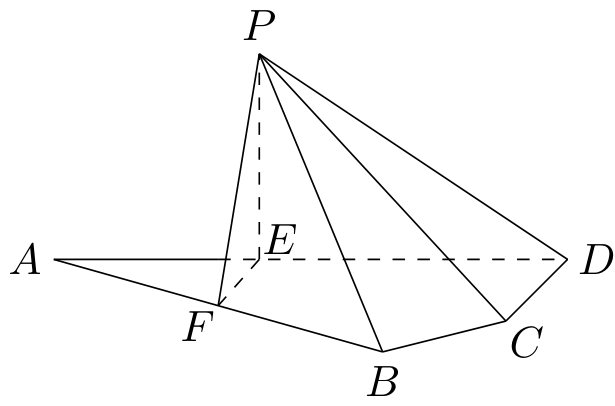
\includegraphics[width=7.6cm]{GaoKao/images/2024/new_gaokao_paper_2/q17_fig1.png}
\par}

        \begin{enumerate}[label=(\arabic*)]
            \item 证明：$EF\perp PD$；
            \item 求面 $PCD$ 与面 $PBF$ 所成的二面角的正弦值．
        \end{enumerate}

        \item （17分）

        某投篮比赛分为两个阶段，每个参赛队由两名队员组成．比赛具体规则如下：第一阶段由参赛队中一名队员投篮3次，若3次都未投中，则该队被淘汰，比赛成绩为0分；若至少投中1次，则该队进入第二阶段．第二阶段由该队的另一名队员投篮3次，每次投篮投中得5分，未投中得0分．该队的比赛成绩为第二阶段的得分总和．某参赛队由甲、乙两名队员组成，设甲每次投中的概率为 $p$，乙每次投中的概率为 $q$，各次投中与否相互独立．

        \begin{enumerate}[label=(\arabic*)]
            \item 若 $p=0.4$，$q=0.5$，甲参加第一阶段比赛，求甲、乙所在队的比赛成绩不少于5分的概率；
            \item 假设 $0<p<q$．
            \begin{enumerate}[label=\textcircled{\arabic*}]
                \item 为使得甲、乙所在队的比赛成绩为15分的概率最大，应该由谁参加第一阶段比赛？
                \item 为使得甲、乙所在队的比赛成绩的数学期望最大，应该由谁参加第一阶段比赛？
            \end{enumerate}
        \end{enumerate}

        \item （17分）

        已知双曲线 $C:x^2-y^2=m\,(m>0)$，点 $P_1(5,4)$ 在 $C$ 上，$k$ 为常数，$0<k<1$．按照如下方式依次构造点 $P_n\,(n=2,3,\cdots)$：过点 $P_{n-1}$ 作斜率为 $k$ 的直线与 $C$ 的左支交于点 $Q_{n-1}$，令 $P_n$ 为 $Q_{n-1}$ 关于 $y$ 轴的对称点．记 $P_n$ 的坐标为 $(x_n,y_n)$．

        \begin{enumerate}[label=(\arabic*)]
            \item 若 $k=\dfrac{1}{2}$，求 $x_2,y_2$；
            \item 证明：数列 $\{x_n-y_n\}$ 是公比为 $\dfrac{1+k}{1-k}$ 的等比数列；
            \item 设 $S_n$ 为 $\triangle P_nP_{n+1}P_{n+2}$ 的面积．证明：对于任意正整数 $n$，$S_n=S_{n+1}$．
        \end{enumerate}
    \end{enumerate}
\end{description}
\clearpage


\subsection{2024年北京卷}\label{gk:2024年北京卷}

\begin{description}
    \item[一、选择题] 本题共10小题，每小题4分，共40分．在每小题给出的四个选项中，选出符合题目要求的一项．
    \begin{enumerate}[leftmargin=5pt]
        \item 已知集合 $M=\{x\mid -3<x<1\}$，$N=\{x\mid -1\leqslant x<4\}$，则 $M\cup N=$
       
        {\centering\begin{tabular*}{\linewidth}{@{}@{\extracolsep{\fill}}llll@{}}
          \(\text{A. }\{x\mid -1\leqslant x<1\}\)  & \(\text{B. }\{x\mid x>-3\}\)  & \(\text{C. }\{x\mid -3<x<4\}\)  & \(\text{D. }\{x\mid x<4\}\)
        \end{tabular*}\par}

        \item 若复数 $z$ 满足 $\dfrac{z}{\i}=-1-\i$，则 $z=$
       
        {\centering\begin{tabular*}{\linewidth}{@{}@{\extracolsep{\fill}}llll@{}}
          \(\text{A. }-1-\i\)  & \(\text{B. }-1+\i\)  & \(\text{C. }1-\i\)  & \(\text{D. }1+\i\)
        \end{tabular*}\par}

        \item 圆 $x^2+y^2-2x+6y=0$ 的圆心到直线 $x-y+2=0$ 的距离为
       
        {\centering\begin{tabular*}{\linewidth}{@{}@{\extracolsep{\fill}}llll@{}}
          \(\text{A. }\sqrt{2}\)  & \(\text{B. }2\)  & \(\text{C. }3\)  & \(\text{D. }3\sqrt{2}\)
        \end{tabular*}\par}

        \item 在 $(x-\sqrt{x})^4$ 的展开式中，$x^3$ 的系数为
       
        {\centering\begin{tabular*}{\linewidth}{@{}@{\extracolsep{\fill}}llll@{}}
          \(\text{A. }6\)  & \(\text{B. }-6\)  & \(\text{C. }12\)  & \(\text{D. }-12\)
        \end{tabular*}\par}

        \item 设 $\bm a,\bm b$ 是向量，则"$(\bm a+\bm b)\cdot(\bm a-\bm b)=0$"是"$\bm a=-\bm b$ 或 $\bm a=\bm b$"的
       
        {\centering\begin{tabular*}{\linewidth}{@{}@{\extracolsep{\fill}}llll@{}}
          \(\text{A. }\)充分不必要条件  & \(\text{B. }\)必要不充分条件  & \(\text{C. }\)充要条件  & \(\text{D. }\)既不充分也不必要条件
        \end{tabular*}\par}

        \item 设函数 $f(x)=\sin\omega x\,(\omega>0)$．已知 $f(x_1)=-1$，$f(x_2)=1$，且 $|x_1-x_2|$ 的最小值为 $\dfrac{\pi}{2}$，则 $\omega=$
       
        {\centering\begin{tabular*}{\linewidth}{@{}@{\extracolsep{\fill}}llll@{}}
          \(\text{A. }1\)  & \(\text{B. }2\)  & \(\text{C. }3\)  & \(\text{D. }4\)
        \end{tabular*}\par}

        \item 生物丰富度指数 $d=\dfrac{S-1}{\ln N}$ 是河流水质的一个评价指标，其中 $S,N$ 分别表示河流中的生物种类数与生物个体总数．生物丰富度指数 $d$ 越大，水质越好．如果某河流治理前后的生物种类数 $S$ 没有变化，生物个体总数由 $N_1$ 变为 $N_2$，生物丰富度指数由 $2.1$ 提高到 $3.15$，则
       
        {\centering\begin{tabular*}{\linewidth}{@{}@{\extracolsep{\fill}}llll@{}}
          \(\text{A. }3N_2=2N_1\)  & \(\text{B. }2N_2=3N_1\)  & \(\text{C. }N_2^2=N_1^3\)  & \(\text{D. }N_2^3=N_1^2\)
        \end{tabular*}\par}

        \item 如图，在四棱锥 $P$-$ABCD$ 中，底面 $ABCD$ 是边长为 $4$ 的正方形，$PA=PB=4$，$PC=PD=2\sqrt{2}$．该棱锥的高为
        
        {\centering
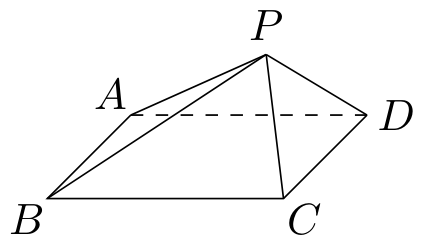
\includegraphics[width=5.3cm]{GaoKao/images/2024/beijing/q8_fig1.png}
\par}

        {\centering\begin{tabular*}{\linewidth}{@{}@{\extracolsep{\fill}}llll@{}}
          \(\text{A. }1\)  & \(\text{B. }2\)  & \(\text{C. }\sqrt{2}\)  & \(\text{D. }\sqrt{3}\)
        \end{tabular*}\par}

        \item 已知 $(x_1,y_1),(x_2,y_2)$ 是函数 $y=2^x$ 的图象上两个不同的点，则
       
        {\centering\begin{tabular*}{\linewidth}{@{}@{\extracolsep{\fill}}llll@{}}
          \(\text{A. }\log_2\dfrac{y_1+y_2}{2}<\dfrac{x_1+x_2}{2}\)  & \(\text{B. }\log_2\dfrac{y_1+y_2}{2}>\dfrac{x_1+x_2}{2}\) \\
          \(\text{C. }\log_2\dfrac{y_1+y_2}{2}<x_1+x_2\)  & \(\text{D. }\log_2\dfrac{y_1+y_2}{2}>x_1+x_2\)
        \end{tabular*}\par}

        \item 已知 $M=\{(x,y)\mid y=x+t(x^2-x),\;1\leqslant x\leqslant2,\;0\leqslant t\leqslant1\}$ 是平面直角坐标系中的点集．设 $d$ 是 $M$ 中两点间的距离的最大值，$S$ 是 $M$ 表示的图形的面积，则
       
        {\centering\begin{tabular*}{\linewidth}{@{}@{\extracolsep{\fill}}llll@{}}
          \(\text{A. }d=3,S<1\)  & \(\text{B. }d=3,S>1\)  & \(\text{C. }d=\sqrt{10},S<1\)  & \(\text{D. }d=\sqrt{10},S>1\)
        \end{tabular*}\par}
    \end{enumerate}
\end{description}

\begin{description}
    \item[二、填空题] 本题共5小题，每小题5分，共25分．
    \begin{enumerate}[leftmargin=5pt]
      \addtocounter{enumi}{+10}
        \item 抛物线 $y^2=16x$ 的焦点坐标为 \rule[-0.3ex]{3em}{0.4pt}．
        \item 在平面直角坐标系 $xOy$ 中，角 $\alpha$ 与角 $\beta$ 均以 $Ox$ 为始边，它们的终边关于原点对称．若 $\alpha\in\bigl[\frac{\pi}{6},\frac{\pi}{3}\bigr]$，则 $\cos\beta$ 的最大值为 \rule[-0.3ex]{3em}{0.4pt}．
        \item 若直线 $y=k(x-3)$ 与双曲线 $\dfrac{x^2}{4}-y^2=1$ 只有一个公共点，则 $k$ 的一个取值为 \rule[-0.3ex]{3em}{0.4pt}．
        \item 汉代刘歆设计的"铜嘉量"是龠、合、升、斗、斛五量合一的标准量器，其中升量器、斗量器、斛量器的形状均可视为圆柱．若升、斗、斛量器的容积成公比为 $10$ 的等比数列，底面直径依次为 $65\,\text{mm}$，$325\,\text{mm}$，$325\,\text{mm}$，且斛量器的高为 $230\,\text{mm}$，则斗量器的高为 \rule[-0.3ex]{3em}{0.4pt} mm，升量器的高为 \rule[-0.3ex]{3em}{0.4pt} mm．（不计量器的厚度）
        \item 设 $\{a_n\}$ 与 $\{b_n\}$ 是两个不同的无穷数列，且都不是常数列．记集合 $M=\{k\mid a_k=b_k,k\in\mathbb{N}^*\}$，给出下列四个结论：

        \ding{172}若 $\{a_n\}$ 与 $\{b_n\}$ 均为等差数列，则 $M$ 中最多有 $1$ 个元素；
        
        \ding{173}若 $\{a_n\}$ 与 $\{b_n\}$ 均为等比数列，则 $M$ 中最多有 $2$ 个元素；
        
        \ding{174}若 $\{a_n\}$ 为等差数列，$\{b_n\}$ 为等比数列，则 $M$ 中最多有 $3$ 个元素；
        
        \ding{175}若 $\{a_n\}$ 为递增数列，$\{b_n\}$ 为递减数列，则 $M$ 中最多有 $1$ 个元素．
        
        其中正确结论的序号是 \rule[-0.3ex]{3em}{0.4pt}．
    \end{enumerate}
\end{description}

\begin{description}
    \item[三、解答题] 本题共6小题，共85分．解答应写出文字说明、证明过程或演算步骤．
    \begin{enumerate}[leftmargin=5pt]
      \addtocounter{enumi}{+15}
        \item （13分）

        在 $\triangle ABC$ 中，$\angle A$ 为钝角，$a=7$，$\sin2B=\dfrac{\sqrt{3}}{7}b\cos B$．

        \begin{enumerate}[label=(\arabic*)]
            \item 求 $\angle A$；
            \item 再从条件\ding{172}、条件\ding{173}、条件\ding{174}这三个条件中选择一个作为已知，使得 $\triangle ABC$ 存在，求 $\triangle ABC$ 的面积．
            \begin{quote}
            条件\ding{172}：$b=7$；条件\ding{173}：$\cos B=\dfrac{13}{14}$；条件\ding{174}：$c\sin A=\dfrac{5\sqrt{3}}{2}$．
            \end{quote}
            注：如果选择的条件不符合要求，第(2)问得0分；如果选择多个符合要求的条件分别解答，按第一个解答计分．
        \end{enumerate}

        \item （14分）

        如图，在四棱锥 $P$-$ABCD$ 中，$BC\parallel AD$，$AB=BC=1$，$AD=3$．点 $E$ 在 $AD$ 上，且 $PE\perp AD$，$PE=DE=2$．

        {\centering
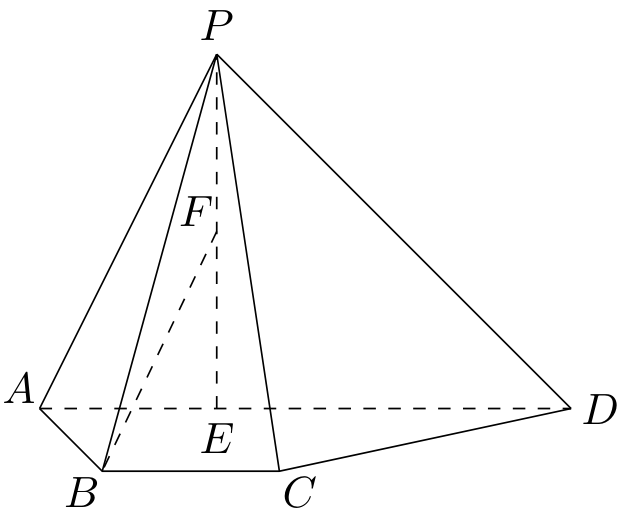
\includegraphics[width=7.8cm]{GaoKao/images/2024/beijing/q17_fig1.png}
\par}

        \begin{enumerate}[label=(\arabic*)]
            \item 若 $F$ 为线段 $PE$ 的中点，求证：$BF\parallel$ 平面 $PCD$；
            \item 若 $AB\perp$ 平面 $PAD$，求平面 $PAB$ 与平面 $PCD$ 夹角的余弦值．
        \end{enumerate}

        \item （14分）

        某保险公司为了解该公司某种保险产品的索赔情况，从合同保险期限届满的保单中随机抽取1000份，记录并整理这些保单的索赔情况，获得数据如下表：

        {\centering\begin{tabular}{c|c|c|c|c|c}
        \hline
        索赔次数 & 0 & 1 & 2 & 3 & 4 \\
        \hline
        保单份数 & 800 & 100 & 60 & 30 & 10 \\
        \hline
        \end{tabular}\par}

        假设：一份保单的保费为 $0.4$ 万元；前三次索赔时，保险公司每次赔偿 $0.8$ 万元；第四次索赔时，保险公司赔偿 $0.6$ 万元．假设不同保单的索赔次数相互独立．用频率估计概率．

        \begin{enumerate}[label=(\arabic*)]
            \item 估计一份保单索赔次数不少于 $2$ 的概率；
            \item 一份保单的毛利润定义为这份保单的保费与赔偿总金额之差．
            \begin{enumerate}[label=\textcircled{\arabic*}]
                \item 记 $X$ 为一份保单的毛利润，估计 $X$ 的数学期望 $EX$；
                \item 如果无索赔的保单的保费减少 $4\%$，有索赔的保单的保费增加 $20\%$，试比较这种情况下一份保单毛利润的数学期望估计值与\ding{172}中 $EX$ 估计值的大小．（结论不要求证明）
            \end{enumerate}
        \end{enumerate}

        \item （15分）

        已知椭圆 $E:\dfrac{x^2}{a^2}+\dfrac{y^2}{b^2}=1\,(a>b>0)$，以椭圆 $E$ 的焦点和短轴端点为顶点的四边形是边长为 $2$ 的正方形．过点 $(0,t)\,(t>\sqrt{2})$ 且斜率存在的直线与椭圆 $E$ 交于不同的两点 $A,B$，过点 $A$ 和 $C(0,1)$ 的直线 $AC$ 与椭圆 $E$ 的另一个交点为 $D$．

        \begin{enumerate}[label=(\arabic*)]
            \item 求椭圆 $E$ 的方程及离心率；
            \item 若直线 $BD$ 的斜率为 $0$，求 $t$ 的值．
        \end{enumerate}

        \item （15分）

        设函数 $f(x)=x+k\ln(1+x)\,(k\neq0)$，直线 $l$ 是曲线 $y=f(x)$ 在点 $(t,f(t))\,(t>0)$ 处的切线．

        \begin{enumerate}[label=(\arabic*)]
            \item 当 $k=-1$ 时，求 $f(x)$ 的单调区间；
            \item 求证：$l$ 不经过点 $(0,0)$；
            \item 当 $k=1$ 时，设点 $A(t,f(t))\,(t>0)$，$C(0,f(t))$，$O(0,0)$，$B$ 为 $l$ 与 $y$ 轴的交点，$S_{\triangle ACO}$ 与 $S_{\triangle ABO}$ 分别表示 $\triangle ACO$ 与 $\triangle ABO$ 的面积．是否存在点 $A$ 使得 $2S_{\triangle ACO}=15S_{\triangle ABO}$ 成立？若存在，这样的点 $A$ 有几个？（参考数据：$1.09<\ln3<1.10$，$1.60<\ln5<1.61$，$1.94<\ln7<1.95$）
        \end{enumerate}

        \item （15分）

        已知集合 $M=\{(i,j,k,w)\mid i\in\{1,2\},j\in\{3,4\},k\in\{5,6\},w\in\{7,8\}$，且 $i+j+k+w$ 为偶数$\}$．

        给定数列 $A:a_1,a_2,\cdots,a_8$ 和序列 $\Omega:T_1,T_2,\cdots,T_s$，其中 $T_t=(i_t,j_t,k_t,w_t)\in M\,(t=1,2,\cdots,s)$，对数列 $A$ 进行如下变换：将 $A$ 的第 $i_1,j_1,k_1,w_1$ 项均加 $1$，其余项不变，得到的数列记作 $T_1(A)$；将 $T_1(A)$ 的第 $i_2,j_2,k_2,w_2$ 项均加 $1$，其余项不变，得到的数列记作 $T_2T_1(A)$；$\cdots$；以此类推，得到数列 $T_s\cdots T_2T_1(A)$，简记为 $\Omega(A)$．

        \begin{enumerate}[label=(\arabic*)]
            \item 给定数列 $A:1,3,2,4,6,3,1,9$ 和序列 $\Omega:(1,3,5,7),(2,4,6,8),(1,3,5,7)$，写出 $\Omega(A)$；
            \item 是否存在序列 $\Omega$，使得 $\Omega(A)$ 为 $a_1+2,a_2+6,a_3+4,a_4+2,a_5+8,a_6+2,a_7+4,a_8+4$？若存在，写出一个 $\Omega$；若不存在，说明理由；
            \item 若数列 $A$ 的各项均为正整数，且 $a_1+a_3+a_5+a_7$ 为偶数，求证："存在序列 $\Omega$，使得 $\Omega(A)$ 的各项都相等"的充要条件为"$a_1+a_2=a_3+a_4=a_5+a_6=a_7+a_8$"．
        \end{enumerate}
    \end{enumerate}
\end{description}
\clearpage


\subsection{2024年上海卷}\label{gk:2024年上海卷}

\begin{description}
    \item[一、填空题] 本大题共有12题，满分54分，第1\textasciitilde6题每题4分，第7\textasciitilde12题每题5分．
    \begin{enumerate}[leftmargin=5pt]
        \item 已知全集 $U=\{1,2,3,4,5\}$，若集合 $A=\{2,4\}$，则 $\overline{A}=$ \rule[-0.3ex]{3em}{0.4pt}．
        \item 已知函数 $y=f(x)$ 的表达式为 $f(x)=\begin{cases}\sqrt{x},&x>0,\\1,&x\leqslant0,\end{cases}$ 则 $f(3)=$ \rule[-0.3ex]{3em}{0.4pt}．
        \item 设 $x\in\mathbb{R}$，不等式 $x^2-2x-3<0$ 的解集为 \rule[-0.3ex]{3em}{0.4pt}．
        \item 设 $a$ 为常数，若函数 $y=x^3+a$ 是奇函数，则 $a=$ \rule[-0.3ex]{3em}{0.4pt}．
        \item 设 $k\in\mathbb{R}$，向量 $\overrightarrow{a}=(2,5)$，$\overrightarrow{b}=(6,k)$．若 $\overrightarrow{a}\parallel\overrightarrow{b}$，则 $k=$ \rule[-0.3ex]{3em}{0.4pt}．
        \item 在 $(x+1)^n$ 的二项展开式中，若各项系数和为 $32$，则 $x^2$ 项的系数为 \rule[-0.3ex]{3em}{0.4pt}．
        \item 若抛物线 $y^2=4x$ 上一点 $P$ 到其准线的距离为 $9$，则点 $P$ 到 $x$ 轴的距离为 \rule[-0.3ex]{3em}{0.4pt}．
        \item 小王参加知识竞赛，题库中A组题有5000道，B组题有4000道，C组题有3000道，若小王做对这三组题的概率依次为0.92、0.86、0.72，则随机从题库中抽取一道题，小王做对的概率是 \rule[-0.3ex]{3em}{0.4pt}．
        \item 设 $m\in\mathbb{R}$，若虚数 $z$ 的实部为 $1$，且满足 $z+\dfrac{2}{z}=m$，则 $m=$ \rule[-0.3ex]{3em}{0.4pt}．
        \item 已知某集合中的元素是不重复的数字组成的三位正整数，若该集合中任意两个数的积均为偶数，则该集合的元素个数的最大值为 \rule[-0.3ex]{3em}{0.4pt}．
        \item 海上有灯塔 $O,A,B$ 和船只 $T$，$A$ 在 $O$ 的正东方向，$B$ 在 $O$ 的正北方向，$A,B$ 到 $O$ 的距离相等，$O,A,T,B$ 按逆时针排列．若 $\angle ATO=37^\circ$，$\angle BTO=16.5^\circ$，则 $\angle BOT=$ \rule[-0.3ex]{3em}{0.4pt}．（结果精确到 $0.1$ 度）
        
        {\centering
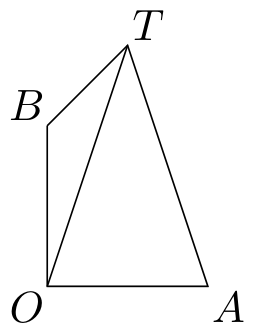
\includegraphics[width=3.1cm]{GaoKao/images/2024/shanghai/q11_fig1.png}
\par}

        \item 等比数列 $\{a_n\}$ 满足首项 $a_1>0$，公比 $q>1$，$I_n=\{x-y\mid x,y\in[a_1,a_2]\cup[a_n,a_{n+1}]\}$，若对任意正整数 $n$，$I_n$ 都是闭区间，则 $q$ 的取值范围是 \rule[-0.3ex]{3em}{0.4pt}．
    \end{enumerate}
\end{description}

\begin{description}
    \item[二、选择题] 本题共4小题，每小题5分，共20分．
    \begin{enumerate}[leftmargin=5pt]
      \addtocounter{enumi}{+12}
        \item 若气温（单位：$^\circ\text{C}$）和海水表层温度（单位：摄氏度）的相关系数为正数，则下列关于两者关系的说法正确的是
       
        {\centering\begin{tabular*}{\linewidth}{@{}@{\extracolsep{\fill}}llll@{}}
          \(\text{A. }\)随着气温由低变高，海水表层温度由低变高 \\
          \(\text{B. }\)随着气温由低变高，海水表层温度由高变低 \\
          \(\text{C. }\)随着气温由低变高，海水表层温度有由低变高的趋势 \\
          \(\text{D. }\)随着气温由低变高，海水表层温度有由高变低的趋势
        \end{tabular*}\par}

        \item 下列函数中，最小正周期是 $2\pi$ 的是
        
        {\centering\begin{tabular*}{\linewidth}{@{}@{\extracolsep{\fill}}llll@{}}
          \(\text{A. }y=\sin x+\cos x\)  & \(\text{B. }y=\sin x\cos x\)  & \(\text{C. }y=\sin^2x+\cos^2x\)  & \(\text{D. }y=\sin^2x-\cos^2x\)
        \end{tabular*}\par}

        \item 已知空间直角坐标系 $Oxyz$ 中的点集 $\Omega$，对任意的 $P_1,P_2,P_3\in\Omega$，均存在不全为 $0$ 的实数 $\lambda_1,\lambda_2,\lambda_3$ 满足 $\lambda_1\overrightarrow{OP_1}+\lambda_2\overrightarrow{OP_2}+\lambda_3\overrightarrow{OP_3}=\overrightarrow{0}$．若 $(1,0,0)\in\Omega$，则 $(0,0,1)\notin\Omega$ 的一个充分条件是
        
        {\centering\begin{tabular*}{\linewidth}{@{}@{\extracolsep{\fill}}llll@{}}
          \(\text{A. }(0,0,0)\in\Omega\)  & \(\text{B. }(-1,0,0)\in\Omega\)  & \(\text{C. }(0,-1,0)\in\Omega\)  & \(\text{D. }(0,0,-1)\in\Omega\)
        \end{tabular*}\par}

        \item 已知定义在 $\mathbb{R}$ 上的函数 $y=f(x)$，$M=\{x_0\mid\text{对任意 }x\in(-\infty,x_0),f(x)<f(x_0)\}$，对于使得 $M=[-1,1]$ 的函数 $y=f(x)$，以下说法正确的是
        
        {\centering\begin{tabular*}{\linewidth}{@{}@{\extracolsep{\fill}}llll@{}}
          \(\text{A. }\)存在 $y=f(x)$ 是偶函数 \\
          \(\text{B. }\)存在 $y=f(x)$ 在 $x=2$ 处取得最大值 \\
          \(\text{C. }\)存在 $y=f(x)$ 是严格增函数 \\
          \(\text{D. }\)存在 $y=f(x)$ 在 $x=-1$ 处取得极小值
        \end{tabular*}\par}
    \end{enumerate}
\end{description}

\begin{description}
    \item[三、解答题] 本题共5小题，共76分．
    \begin{enumerate}[leftmargin=5pt]
      \addtocounter{enumi}{+16}
        \item （14分）

        如图，在正四棱锥 $P$-$ABCD$ 中，$O$ 为底面 $ABCD$ 的中心．

        {\centering
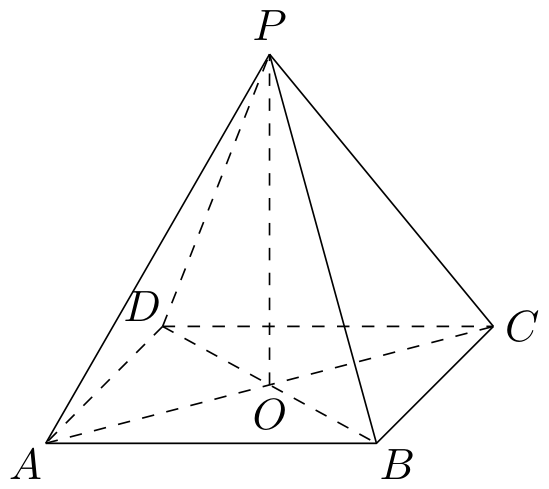
\includegraphics[width=6.6cm]{GaoKao/images/2024/shanghai/q17_fig1.png}
\par}

        \begin{enumerate}[label=(\arabic*)]
            \item 若 $AP=5$，$AD=3\sqrt{2}$，将 $\triangle POA$ 绕直线 $PO$ 旋转一周，求所得旋转体的体积；
            \item 若 $AP=AD$，$E$ 为 $PB$ 的中点，求直线 $BD$ 与平面 $AEC$ 所成角的大小．
        \end{enumerate}

        \item （14分）

        已知 $f(x)=\log_a x\,(a>0$ 且 $a\neq1)$．

        \begin{enumerate}[label=(\arabic*)]
            \item 若函数 $y=f(x)$ 的图象过点 $(4,2)$，求 $f(2x-2)<f(x)$ 的解集；
            \item 若存在 $x$ 使 $f(x+1)$、$f(ax)$、$f(x+2)$ 依次成等差数列，求 $a$ 的取值范围．
        \end{enumerate}

        \item （14分）

        某地区为调查初中学生体育锻炼时长与学业成绩的关系，从该地区29000名初中生抽取580人，得到日均体育锻炼时长（表中简称时长）与学业成绩的数据如下表所示：

        {\centering\begin{tabular}{c|c|c|c|c|c|c}
        \hline
        时长 & $[0,0.5)$ & $[0.5,1)$ & $[1,1.5)$ & $[1.5,2)$ & $[2,2.5)$ & 合计 \\
        \hline
        优秀 & 5 & 44 & 42 & 3 & 1 & 95 \\
        \hline
        不优秀 & 134 & 147 & 137 & 40 & 27 & 485 \\
        \hline
        合计 & 139 & 191 & 179 & 43 & 28 & 580 \\
        \hline
        \end{tabular}\par}

        \begin{enumerate}[label=(\arabic*)]
            \item 估计该地区29000名初中生中体育锻炼时长大于1小时人数；
            \item 估计该地区初中生平均日均体育锻炼时长；（结果精确到0.1小时）
            \item 判断是否有 $95\%$ 的把握认为该地区初中生学业成绩优秀与日均体育锻炼时长不小于1小时且小于2小时有关？
            
            \begin{quote}
            $\chi^2=\dfrac{n(ad-bc)^2}{(a+b)(c+d)(a+c)(b+d)}$，其中 $n=a+b+c+d$，$P(\chi^2\geqslant3.841)\approx0.05$．
            \end{quote}
        \end{enumerate}

        \item （17分）

        双曲线 $\Gamma:x^2-\dfrac{y^2}{b^2}=1\,(b>0)$，左、右顶点分别为 $A_1,A_2$，过点 $M(-2,0)$ 的直线交 $\Gamma$ 于两点 $P,Q$ 两点．

        \begin{enumerate}[label=(\arabic*)]
            \item 若离心率 $e=2$，求 $b$ 的值；
            \item 若 $b=\dfrac{2\sqrt{6}}{3}$，点 $P$ 在第一象限，$\triangle MA_2P$ 为等腰三角形，求点 $P$ 的坐标；
            \item 连接 $QO$（$O$ 为坐标原点）并延长交 $\Gamma$ 于点 $R$，若 $\overrightarrow{A_1R}\cdot\overrightarrow{A_2P}=1$，求 $b$ 的取值范围．
        \end{enumerate}

        \item （17分）

        设 $D$ 是 $\mathbb{R}$ 的一个非空子集，$y=f(x)$ 是定义在 $D$ 上的函数．对于点 $M(a,b)$，记 $s(x)=(x-a)^2+(f(x)-b)^2$，若对于点 $P(x_0,f(x_0))$，满足函数 $y=s(x)$ 在 $x=x_0$ 处取得最小值，则称 $P$ 是 $M$ 的 $f$ 最近点．

        \begin{enumerate}[label=(\arabic*)]
            \item $f(x)=\dfrac{1}{x}$，$M(0,0)$，$D=(0,+\infty)$，求证：存在 $M$ 的 $f$ 最近点；
            \item $f(x)=\mathrm{e}^x$，$M(1,0)$，$D=\mathbb{R}$，若曲线 $y=f(x)$ 上一点 $P$ 满足 $MP$ 垂直于 $y=f(x)$ 在点 $P(x_0,f(x_0))$ 处的切线，则 $P$ 是否为 $M$ 的 $f$ 最近点？
            \item 已知 $D=\mathbb{R}$，$y=f(x)$ 的导函数为 $y=f'(x)$，$y=g(x)$ 在 $\mathbb{R}$ 上的函数值恒正．对任意 $t\in\mathbb{R}$，点 $M_1$ 的坐标为 $(t-1,f(t)-g(t))$，点 $M_2$ 的坐标为 $(t+1,f(t)+g(t))$，若对任意的 $t\in\mathbb{R}$，总存在 $y=f(x)$ 上一点 $P$，使得 $P$ 既是 $M_1$ 的 $f$ 最近点，又是 $M_2$ 的 $f$ 最近点，试求 $y=f(x)$ 的单调性．
        \end{enumerate}
    \end{enumerate}
\end{description}
\clearpage


\subsection{2024年天津卷}\label{gk:2024年天津卷}

\begin{description}
    \item[一、选择题] 本题共9小题，每小题5分，共45分．在每小题给出的四个选项中，只有一项是符合题目要求的．
    \begin{enumerate}[leftmargin=5pt]
        \item 已知集合 $A=\{1,2,3,4\}$，$B=\{2,3,4,5\}$，则 $A\cap B=$
       
        {\centering\begin{tabular*}{\linewidth}{@{}@{\extracolsep{\fill}}llll@{}}
          \(\text{A. }\{1,2,3,4\}\)  & \(\text{B. }\{2,3,4\}\)  & \(\text{C. }\{2,4\}\)  & \(\text{D. }\{1\}\)
        \end{tabular*}\par}

        \item 已知 $a,b\in\mathbb{R}$，则"$a^3=b^3$"是"$3^a=3^b$"的
       
        {\centering\begin{tabular*}{\linewidth}{@{}@{\extracolsep{\fill}}llll@{}}
          \(\text{A. }\)充分不必要条件  & \(\text{B. }\)必要不充分条件  & \(\text{C. }\)充要条件  & \(\text{D. }\)既不充分也不必要条件
        \end{tabular*}\par}

        \item 下列图中，相关性系数最大的是
        
        {\centering
            \begin{tabular*}{\linewidth}{@{}@{\extracolsep{\fill}}cccc@{}}
            \(\text{A. }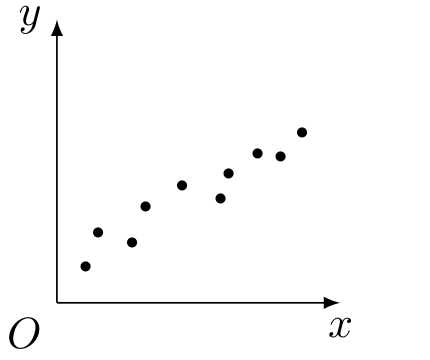
\includegraphics[width=0.15\paperwidth]{GaoKao/images/2024/tianjin/q3_fig1.png}\)  &  \(\text{B. }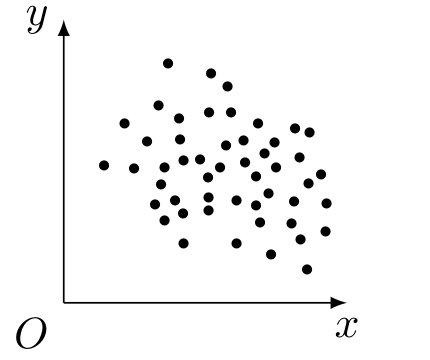
\includegraphics[width=0.15\paperwidth]{GaoKao/images/2024/tianjin/q3_fig2.png}\)  &  \(\text{C. }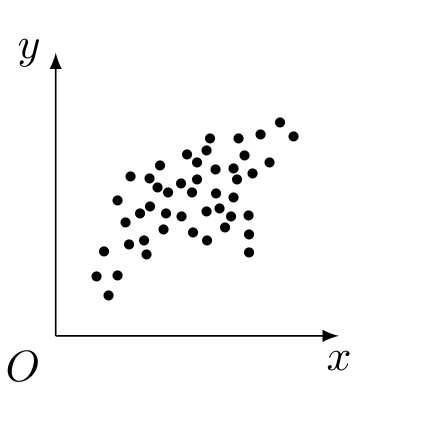
\includegraphics[width=0.15\paperwidth]{GaoKao/images/2024/tianjin/q3_fig3.png}\)  &  \(\text{D. }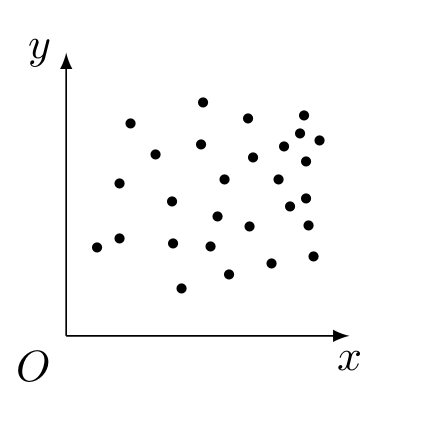
\includegraphics[width=0.15\paperwidth]{GaoKao/images/2024/tianjin/q3_fig4.png}\)
        \end{tabular*}
        \par}

        \item 下列函数是偶函数的为
       
        {\centering\begin{tabular*}{\linewidth}{@{}@{\extracolsep{\fill}}llll@{}}
          \(\text{A. }y=\dfrac{\mathrm{e}^x-x^2}{\mathrm{e}^x+x^2}\)  & \(\text{B. }y=\dfrac{\cos x-x^2}{x^2+1}\)  & \(\text{C. }y=\dfrac{\mathrm{e}^x-x}{\mathrm{e}^x+x}\)  & \(\text{D. }y=\dfrac{\sin x-x}{x^2+1}\)
        \end{tabular*}\par}

        \item 设 $a=4.2^{-0.2}$，$b=4.2^{0.2}$，$c=\log_{4.2}0.2$，则 $a,b,c$ 的大小关系为
       
        {\centering\begin{tabular*}{\linewidth}{@{}@{\extracolsep{\fill}}llll@{}}
          \(\text{A. }a<b<c\)  & \(\text{B. }a<c<b\)  & \(\text{C. }c<b<a\)  & \(\text{D. }c<a<b\)
        \end{tabular*}\par}

        \item 已知 $m,n$ 是两条直线，$\alpha$ 是一个平面．下列命题正确的是
       
        {\centering\begin{tabular*}{\linewidth}{@{}@{\extracolsep{\fill}}llll@{}}
          \(\text{A. }\)若 $m\parallel\alpha,m\perp n$，则 $n\perp\alpha$  & \(\text{B. }\)若 $m\perp\alpha,m\perp n$，则 $n\perp\alpha$ \\
          \(\text{C. }\)若 $m\parallel\alpha,n\perp\alpha$，则 $m\perp n$  & \(\text{D. }\)若 $m\perp\alpha,n\perp\alpha$，则 $m\perp n$
        \end{tabular*}\par}

        \item 已知函数 $f(x)=3\sin\bigl(\omega x+\frac{\pi}{3}\bigr)\,(\omega>0)$ 的最小正周期为 $\pi$，则 $f(x)$ 在区间 $\bigl[-\frac{\pi}{12},\frac{\pi}{6}\bigr]$ 上的最小值为
       
        {\centering\begin{tabular*}{\linewidth}{@{}@{\extracolsep{\fill}}llll@{}}
          \(\text{A. }-\dfrac{3\sqrt{3}}{2}\)  & \(\text{B. }-\dfrac{3}{2}\)  & \(\text{C. }0\)  & \(\text{D. }\dfrac{3}{2}\)
        \end{tabular*}\par}

        \item 双曲线 $\dfrac{x^2}{a^2}-\dfrac{y^2}{b^2}=1\,(a>0,b>0)$ 的左、右焦点分别为 $F_1,F_2$，点 $P$ 在双曲线右支上，直线 $PF_2$ 的斜率为 $2$．若 $\triangle PF_1F_2$ 是直角三角形，且面积为 $8$，则双曲线的方程为
       
        {\centering\begin{tabular*}{\linewidth}{@{}@{\extracolsep{\fill}}llll@{}}
          \(\text{A. }\dfrac{x^2}{2}-\dfrac{y^2}{8}=1\)  & \(\text{B. }\dfrac{x^2}{4}-\dfrac{y^2}{8}=1\)  & \(\text{C. }\dfrac{x^2}{8}-\dfrac{y^2}{2}=1\)  & \(\text{D. }\dfrac{x^2}{8}-\dfrac{y^2}{4}=1\)
        \end{tabular*}\par}

        \item 在如图五面体中，棱 $AD,BE,CF$ 互相平行，且两两之间的距离均为 $1$．若 $AD=1$，$BE=2$，$CF=3$，则该五面体的体积为
        
        {\centering
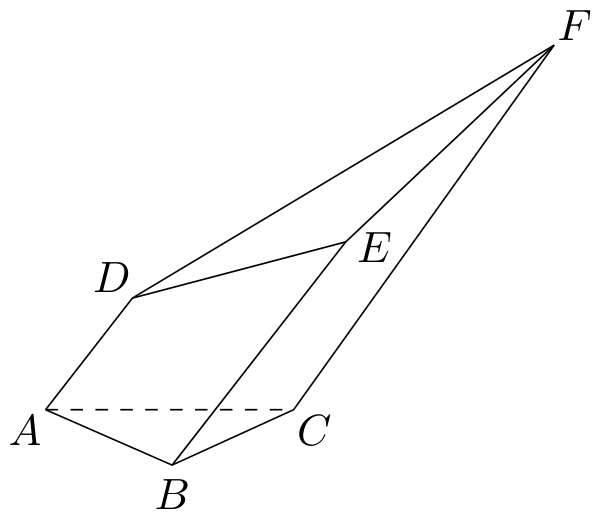
\includegraphics[width=7.5cm]{GaoKao/images/2024/tianjin/q9_fig1.png}
\par}

        {\centering\begin{tabular*}{\linewidth}{@{}@{\extracolsep{\fill}}llll@{}}
          \(\text{A. }\dfrac{\sqrt{3}}{6}\)  & \(\text{B. }\dfrac{\sqrt{3}}{4}+\dfrac{1}{2}\)  & \(\text{C. }\dfrac{\sqrt{3}}{2}\)  & \(\text{D. }\dfrac{3\sqrt{3}}{4}-\dfrac{1}{2}\)
        \end{tabular*}\par}
    \end{enumerate}
\end{description}

\begin{description}
    \item[二、填空题] 本题共6小题，每小题5分，共30分．
    \begin{enumerate}[leftmargin=5pt]
      \addtocounter{enumi}{+9}
        \item $\i$ 是虚数单位，复数 $(\sqrt{5}+\i)(\sqrt{5}-2\i)=$ \rule[-0.3ex]{3em}{0.4pt}．
        \item 在 $\bigl(\dfrac{x^2}{3}+\dfrac{3}{x^2}\bigr)^6$ 的展开式中，常数项为 \rule[-0.3ex]{3em}{0.4pt}．
        \item 已知圆 $(x-1)^2+y^2=25$ 的圆心与抛物线 $y^2=2px$ 的焦点 $F$ 重合，且曲线在第一象限的交点为 $A$，则原点到直线 $AF$ 的距离为 \rule[-0.3ex]{3em}{0.4pt}．
        \item 某校组织学生参加农业实践活动，期间安排了劳动技能比赛，比赛共 $5$ 个项目，分别为整地做畦、旱田播种、作物移栽、田间灌溉、藤架搭建，规定每人参加其中 $3$ 个项目．假设每人参加每个项目的可能性相同，则甲同学参加"整地做畦"项目的概率为 \rule[-0.3ex]{3em}{0.4pt}；已知乙同学参加的 $3$ 个项目中有"整地做畦"，则他还参加"田间灌溉"项目的概率为 \rule[-0.3ex]{3em}{0.4pt}．
        \item 已知正方形 $ABCD$ 的边长为 $1$，$\overrightarrow{DE}=2\overrightarrow{EC}$．若 $\overrightarrow{BE}=\lambda\overrightarrow{BA}+\mu\overrightarrow{BC}$，其中 $\lambda,\mu$ 为实数，则 $\lambda+\mu=$ \rule[-0.3ex]{3em}{0.4pt}；设 $F$ 是线段 $BE$ 上的动点，$G$ 为线段 $AF$ 的中点，则 $\overrightarrow{AF}\cdot\overrightarrow{DG}$ 的最小值为 \rule[-0.3ex]{3em}{0.4pt}．
        \item 设 $a\in\mathbb{R}$，函数 $f(x)=2\sqrt{x^2-ax}-|ax-2|+1$．若 $f(x)$ 恰有一个零点，则 $a$ 的取值范围是 \rule[-0.3ex]{3em}{0.4pt}．
    \end{enumerate}
\end{description}

\begin{description}
    \item[三、解答题] 本题共5小题，共75分．解答应写出文字说明、证明过程或演算步骤．
    \begin{enumerate}[leftmargin=5pt]
      \addtocounter{enumi}{+15}
        \item （14分）

        在 $\triangle ABC$ 中，角 $A,B,C$ 所对的边分别为 $a,b,c$．已知 $\cos B=\dfrac{9}{16}$，$b=5$，$\dfrac{a}{c}=\dfrac{2}{3}$．

        \begin{enumerate}[label=(\arabic*)]
            \item 求 $a$ 的值；
            \item 求 $\sin A$ 的值；
            \item 求 $\cos(B-2A)$ 的值．
        \end{enumerate}

        \item （15分）

        如图，在四棱柱 $ABCD$-$A_1B_1C_1D_1$ 中，$AA_1\perp$ 平面 $ABCD$，$AB\perp AD$，$AB\parallel DC$，$AB=AA_1=2$，$AD=DC=1$，$M,N$ 分别为 $DD_1,B_1C_1$ 的中点．

        {\centering
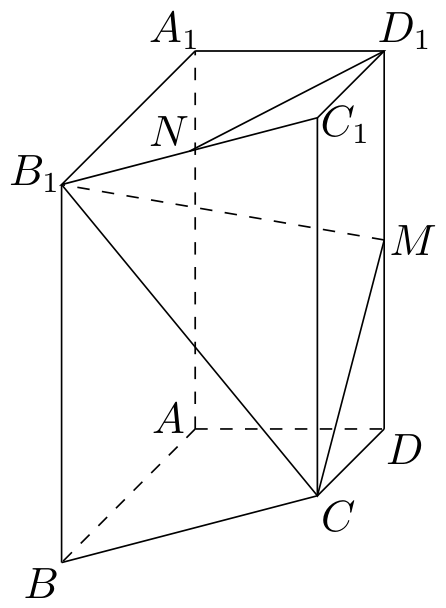
\includegraphics[width=4.5cm]{GaoKao/images/2024/tianjin/q17_fig1.png}
\par}

        \begin{enumerate}[label=(\arabic*)]
            \item 求证：$D_1N\parallel$ 平面 $CB_1M$；
            \item 求平面 $CB_1M$ 与平面 $BB_1C_1C$ 夹角的余弦值；
            \item 求点 $B$ 到平面 $CB_1M$ 的距离．
        \end{enumerate}

        \item （15分）

        已知椭圆 $\dfrac{x^2}{a^2}+\dfrac{y^2}{b^2}=1\,(a>b>0)$ 的离心率为 $\dfrac{1}{2}$．左顶点为 $A$，下顶点为 $B$，点 $C$ 为线段 $OB$ 的中点（$O$ 为原点），$\triangle ABC$ 的面积为 $\dfrac{3\sqrt{3}}{2}$．

        \begin{enumerate}[label=(\arabic*)]
            \item 求椭圆的方程；
            \item 过点 $C$ 的动直线与椭圆相交于 $P,Q$ 两点．在 $y$ 轴上是否存在点 $T$，使得 $\overrightarrow{TP}\cdot\overrightarrow{TQ}\leqslant0$ 恒成立？若存在，求出点 $T$ 纵坐标的取值范围；若不存在，请说明理由．
        \end{enumerate}

        \item （15分）

        已知 $\{a_n\}$ 为公比大于 $0$ 的等比数列，其前 $n$ 项和为 $S_n$，且 $a_1=1$，$S_2=a_3-1$．

        \begin{enumerate}[label=(\arabic*)]
            \item 求 $\{a_n\}$ 的通项公式及 $S_n$；
            \item 设数列 $\{b_n\}$ 满足 $b_n=\begin{cases}k,&n=a_k,\\b_{n-1}+2k,&a_k<n<a_{k+1},\end{cases}$ 其中 $k\in\mathbb{N}^*$．
            \begin{enumerate}[label=\textcircled{\arabic*}]
                \item 求证：当 $n=a_{k+1}\,(k\in\mathbb{N}^*$，且 $k>1)$ 时，$b_{n-1}\geqslant a_kb_n$；
                \item 求 $\displaystyle\sum_{i=1}^{S_n}b_i$．
            \end{enumerate}
        \end{enumerate}

        \item （16分）

        已知函数 $f(x)=x\ln x$．

        \begin{enumerate}[label=(\arabic*)]
            \item 求曲线 $y=f(x)$ 在点 $(1,f(1))$ 处的切线方程；
            \item 若 $f(x)\geqslant a(x-\sqrt{x})$ 对任意 $x\in(0,+\infty)$ 成立，求实数 $a$ 的值；
            \item 若 $x_1,x_2\in(0,1)$，求证：$|f(x_1)-f(x_2)|\leqslant|x_1-x_2|^{\frac{1}{2}}$．
        \end{enumerate}
    \end{enumerate}
\end{description}
\clearpage

